\documentclass[11pt]{article}

\usepackage[T1]{fontenc}
\IfFileExists{libertinus.sty}{\usepackage{libertinus}}{\usepackage{lmodern}}
\usepackage[a4paper,margin=27mm,headheight=15pt]{geometry}
\usepackage{microtype}
\usepackage{amsmath,amssymb,amsthm,mathtools}
% Canonical mathematical notation for active FabiusFunction LaTeX documents.
%
% This file is intentionally a plain TeX input rather than a LaTeX package.
% Every standalone document loads it by an explicit path relative to that
% document's directory; included fragments inherit the definitions from their
% root document.  Keep this file independent of document layout and metadata.
%
% Contract:
%   * one command has one mathematical meaning throughout the active corpus;
%   * names encode semantic roles rather than a document-local choice of letter;
%   * visually similar but differently normalized objects have different print;
%   * every command below is defined normatively in the notation catalogue.
%
% The active corpus excludes docs/archive/.  Historical sources may retain
% their original notation only inside an explicitly labelled quotation.

\makeatletter
\@ifundefined{mathbb}{%
  \PackageError{fabius-notation}{The amssymb package must be loaded first}%
    {Load amsmath and amssymb before inputting fabius-notation.tex.}%
}{}
\@ifundefined{operatorname}{%
  \PackageError{fabius-notation}{The amsmath package must be loaded first}%
    {Load amsmath before inputting fabius-notation.tex.}%
}{}
\makeatother

% Version stamp used by the catalogue and by static audits.
\newcommand{\FabiusNotationVersion}{2026-08-31}

% Number systems.  NaturalNumbers is explicitly the nonnegative convention.
\newcommand{\NaturalNumbers}{\mathbb{N}_{0}}
\newcommand{\PositiveIntegers}{\mathbb{N}_{>0}}
\newcommand{\IntegerNumbers}{\mathbb{Z}}
\newcommand{\RationalNumbers}{\mathbb{Q}}
\newcommand{\RealNumbers}{\mathbb{R}}
\newcommand{\ComplexNumbers}{\mathbb{C}}
\newcommand{\ExtendedRealNumbers}{\overline{\mathbb{R}}}

% The three principal Fabius--Rvachev functions.  Subscripts are deliberate:
% a bare F and a calligraphic F have several unrelated uses in the corpus.
\newcommand{\FabiusBounded}{F_{\mathrm{bd}}}
\newcommand{\FabiusGlobal}{F_{\mathrm{gl}}}
\newcommand{\FabiusQuantile}{Q_{F}}
\newcommand{\FabiusClampedQuantile}{Q_{F,\mathrm{cl}}}
\newcommand{\RvachevUp}{\operatorname{up}}

% Constants, elementary operators, and delimiters.
\newcommand{\EulerE}{\mathrm{e}}
\newcommand{\ImaginaryUnit}{\mathrm{i}}
\newcommand{\Differential}{\mathop{}\!\mathrm{d}}
\newcommand{\AbsoluteValue}[1]{\left\lvert #1\right\rvert}
\newcommand{\Norm}[1]{\left\lVert #1\right\rVert}
\newcommand{\Floor}[1]{\left\lfloor #1\right\rfloor}
\newcommand{\Ceiling}[1]{\left\lceil #1\right\rceil}
\newcommand{\FractionalPart}[1]{\left\{#1\right\}}
\newcommand{\PositivePart}[1]{\left(#1\right)_{+}}
\newcommand{\IndicatorOf}[1]{\mathbf{1}_{#1}}
\newcommand{\SetOf}[1]{\left\{#1\right\}}
\newcommand{\InnerProduct}[1]{\left\langle #1\right\rangle}
\newcommand{\CardinalityOf}[1]{\left\lvert #1\right\rvert}
\newcommand{\DefinitionEquals}{\mathrel{\coloneqq}}
\newcommand{\Sign}{\operatorname{sgn}}
\newcommand{\IdentityOperator}{\operatorname{id}}
\newcommand{\SpanOperator}{\operatorname{span}}
\newcommand{\TraceOperator}{\operatorname{tr}}
\newcommand{\RankOperator}{\operatorname{rank}}
\newcommand{\DiagonalOperator}{\operatorname{diag}}
\newcommand{\ResidueOperator}{\operatorname*{Res}}
\newcommand{\LeastCommonMultiple}{\operatorname{lcm}}
\newcommand{\OrderOperator}{\operatorname{ord}}
\newcommand{\PrincipalLogarithm}{\operatorname{Log}}
\newcommand{\FallingFactorial}[2]{\left(#1\right)^{\underline{#2}}}
\newcommand{\RisingFactorial}[2]{\left(#1\right)^{\overline{#2}}}

% Support, topology, convolution, and metric notation.
\newcommand{\SupportOperator}{\operatorname{supp}}
\newcommand{\SupportOf}[1]{\SupportOperator\!\left(#1\right)}
\newcommand{\TopologicalSupportOf}[1]{\operatorname{tsupp}\!\left(#1\right)}
\newcommand{\Convolution}{\mathbin{*}}
\newcommand{\MetricDistance}{\operatorname{dist}}
\newcommand{\TotalVariationDistance}{d_{\mathrm{TV}}}

% Probability.  Equality and convergence in law are not metric distance.
\newcommand{\Probability}{\mathbb{P}}
\newcommand{\Expectation}{\mathbb{E}}
\newcommand{\Variance}{\operatorname{Var}}
\newcommand{\Covariance}{\operatorname{Cov}}
\newcommand{\LawOperator}{\operatorname{Law}}
\newcommand{\LawOf}[1]{\LawOperator\!\left(#1\right)}
\newcommand{\EqualInLaw}{\mathrel{\overset{\mathrm{law}}{=}}}
\newcommand{\ConvergesInLaw}{\mathrel{\xrightarrow{\mathrm{law}}}}

% Fourier and integral transforms.  The printed labels expose normalization.
% FourierTwoPi uses exp(-2*pi*i*x*xi); FourierAngular uses exp(-i*x*omega).
\newcommand{\FourierTwoPi}[1]{\widehat{#1}_{\,2\pi}}
\newcommand{\FourierAngular}[1]{\widehat{#1}_{\,\mathrm{ang}}}
\newcommand{\LaplaceTransformSymbol}{\mathcal{L}}
\newcommand{\MellinTransformSymbol}{\mathcal{M}}
\newcommand{\LaplaceTransformOf}[1]{\LaplaceTransformSymbol\!\left[#1\right]}
\newcommand{\MellinTransformOf}[1]{\MellinTransformSymbol\!\left[#1\right]}
\newcommand{\MomentGeneratingFunction}[1]{M_{#1}}
\newcommand{\CharacteristicFunction}[1]{\varphi_{#1}}

% The two standard sinc functions must never share one symbol.
\newcommand{\SincRad}{\operatorname{sinc}_{\mathrm{rad}}}
\newcommand{\SincPi}{\operatorname{sinc}_{\pi}}

% Binary arithmetic and Thue--Morse notation.
\newcommand{\BinaryDigitSum}{\operatorname{wt}_{2}}
\newcommand{\ThueMorseSignSymbol}{\varepsilon}
\newcommand{\ThueMorseSign}[1]{\varepsilon_{#1}}
\newcommand{\PadicValuation}[1]{\nu_{#1}}
\newcommand{\TwoAdicValuation}{\nu_{2}}

% q-series notation.  Every base is an explicit argument.
\newcommand{\QPochhammer}[3]{\left(#1;#2\right)_{#3}}
\newcommand{\GaussianBinomial}[3]{%
  \genfrac{[}{]}{0pt}{}{#1}{#2}_{#3}%
}
\newcommand{\QInteger}[2]{\left[#1\right]_{#2}}

% Named special functions.
\newcommand{\Polylogarithm}{\operatorname{Li}}
\newcommand{\LambertW}{W}
\newcommand{\GammaFunction}{\Gamma}
\newcommand{\RiemannZeta}{\zeta}

% Asymptotics.  BigO and LittleO are operator tokens for existing formula
% grammar; prefer the At forms so that the limiting regime is printed.
\newcommand{\BigO}{\mathcal{O}}
\newcommand{\LittleO}{o}
\newcommand{\BigOAt}[2]{\mathcal{O}_{#2}\!\left(#1\right)}
\newcommand{\LittleOAt}[2]{o_{#2}\!\left(#1\right)}

\usepackage{bm}
\usepackage{booktabs,longtable,array,tabularx}
\usepackage{graphicx}
\usepackage{float}
\usepackage{enumitem}
\usepackage{xcolor}
\usepackage{xurl}
\usepackage{hyperref}
\usepackage[nameinlink,capitalise,noabbrev]{cleveref}
\usepackage{url}
\usepackage{listings}
\usepackage{caption}
\usepackage{subcaption}
\usepackage{fancyhdr}
\usepackage{lastpage}

\graphicspath{{figures/}}
\hypersetup{
  colorlinks=true,
  linkcolor=blue!55!black,
  citecolor=green!35!black,
  urlcolor=blue!60!black,
  pdftitle={Jacobi-Digit Deformations of the Fabius--Rvachev Law},
  pdfauthor={Research report prepared for Vladimir Reshetnikov}
}

\pagestyle{fancy}
\setlength{\headheight}{14pt}
\fancyhf{}
\lhead{Jacobi-digit Fabius--Rvachev frontiers}
\rhead{\thepage\ of \pageref*{LastPage}}
\renewcommand{\headrulewidth}{0.4pt}

\setcounter{tocdepth}{2}
\setcounter{secnumdepth}{3}
\allowdisplaybreaks
\emergencystretch=2em

\newtheorem{theorem}{Theorem}[section]
\newtheorem{proposition}[theorem]{Proposition}
\newtheorem{lemma}[theorem]{Lemma}
\newtheorem{corollary}[theorem]{Corollary}
\newtheorem{conjecture}[theorem]{Conjecture}
\newtheorem{problem}[theorem]{Problem}
\theoremstyle{definition}
\newtheorem{definition}[theorem]{Definition}
\newtheorem{experiment}[theorem]{Numerical observation}
\theoremstyle{remark}
\newtheorem{remark}[theorem]{Remark}

\newcommand{\Fab}{\operatorname{Fab}}
\newcommand{\Jcal}{\mathcal{J}}
\newcommand{\Zcal}{\mathcal{Z}}
\newcommand{\Kcal}{\mathcal{K}}
\newcommand{\Bcal}{\mathcal{B}}
\newcommand{\Iop}{\mathsf{I}}
\newcommand{\Dop}{\mathsf{D}}
\newcommand{\Wm}{W_{-1}}
\newcommand{\statusP}{\textcolor{green!35!black}{\textbf{proved here}}}
\newcommand{\statusC}{\textcolor{orange!70!black}{\textbf{conjectural}}}
\newcommand{\statusN}{\textcolor{blue!55!black}{\textbf{numerical}}}
\newcommand{\repo}{\texttt{ProveIt}}

\title{\textbf{Jacobi-Digit Deformations of the Fabius--Rvachev Law}\\[0.35em]
\large Geometric Bessel products, spherical random flights, Rayleigh cumulants,\\
higher-order refinement, and inverse endpoint asymptotics}
\author{Research report prepared for Vladimir Reshetnikov}
\date{30 August 2026}

\begin{document}
\maketitle

\begin{abstract}
This report develops a two-parameter deformation of the normalized
Fabius--Rvachev probability law.  The uniform ``digits'' in the usual
geometric random series are replaced by symmetric beta, equivalently Jacobi,
digits
\[
 \rho_\alpha(u)=
 \frac{\Gamma(\alpha+\tfrac12)}{\sqrt\pi\,\Gamma(\alpha)}
 (1-u^2)^{\alpha-1}\IndicatorOf{(-1,1)}(u),
 \qquad \alpha>0,
\]
and one studies
\[
 X_{q,\alpha}=(1-q)\sum_{n\ge0}q^nU_{\alpha,n},\qquad 0<q<1.
\]
The case \(\alpha=1\) is the geometric-uniform family already developed in
the repository; \(q=1/2,\alpha=1\) is the normalized Rvachev \(\RvachevUp\) law.
The new parameter changes the one-step atom rather than merely the geometric
scale.  It turns the sinc product into an infinite product of normalized
Bessel functions and produces a continuous bridge among Bernoulli
convolutions, arcsine/Bessel cascades, the Rvachev law, spherical random
flights, Jacobi--Gegenbauer polynomials, and Hermite asymptotics.

The principal results proved here are: an exact geometric Bessel-product
formula and super-polynomial Fourier decay; a spherical random-flight model
with an annulus-to-ball support transition; Rayleigh-sum cumulants and Bell
moments with a clean \(q\)-integer factor; an exact Bessel spectral-zeta
factorization; a countable dense set of scale resonances and a generic
simple-zero theorem; a universal Weyl law for the Fourier zeros; finite
higher-order refinement equations for every integer \(\alpha\); an exact
fractional Volterra--pantograph equation at an endpoint; a uniform
Wasserstein-rate desingularization of Bernoulli convolutions; Gaussian limits
along both \(q\uparrow1\) and \(\alpha\to\infty\); and a
Jacobi--Hermite orthogonal-polynomial bridge.  The endpoint small-ball law
implies a new inverse-quantile asymptotic, including the usual inverse Fabius
leading scale as a specialization.

A symbolic/numerical study reveals an unexpected turning transition in the
third monic recurrence coefficient at
\(\alpha_3^*\approx0.066515108060995\).  This phase statement, a complete
Lambert-\(W_{-1}\) endpoint expansion, algebraic nonresonance of Bessel zeros,
and a matrix-valued Thue--Morse generalization are isolated as conjectures or
research programs.  Novelty claims throughout are repository-relative, not
claims of global historical priority.
\end{abstract}

\tableofcontents
\clearpage

\section{Scope, status, and repository audit}

\subsection{Snapshot and audit method}

The final repository comparison in this report is pinned to commit
\begin{center}
\nolinkurl{fdfb6369519e00a2213241ddadf03f7556172134}
\end{center}
\noindent of
\href{https://github.com/VladimirReshetnikov/ProveIt}{\repo}.  At that snapshot,
a GitHub code-index query returned 119 files with extension \texttt{.tex}
under \texttt{Analysis/FabiusFunction/docs}.  The corpus was audited by a
combination of:
\begin{enumerate}[label=(\roman*)]
 \item direct reading of the canonical consolidated volumes, their manifests,
       and the active frontier reports most closely related to the present
       construction;
 \item repository-wide exact searches for the defining phrases and formulas
       of each proposed result; and
 \item specialization checks against the established geometric-uniform,
       sinc-product, endpoint, inverse-Fabius, orthogonal-polynomial, and
       spectral-zeta theories.
\end{enumerate}
The repository moved during the investigation, so a commit hash is essential
for a reproducible ``not already present'' statement.

The nearest existing materials include the canonical exponents and
\(q\)-series volume, the cyclotomic \(q\)-Fabius frontier, the parameter-response
report, the generalized-base atomic-function report, the representation
volume, and the inverse-endpoint reports.  In particular, the repository
already contains the uniform-digit family
\[
 (1-q)\sum_{n\ge0}q^n U_n,\qquad U_n\sim\operatorname{Unif}[-1,1],
\]
its sinc product, Bernoulli cumulants, Bell moments, Gaussian limit,
Legendre-to-Hermite transition, and the dyadic Thue--Morse sign law.  Those
facts are used as consistency checks but are not presented as new results.

\subsection{Novelty crosswalk}

\begin{table}[H]
\centering
\small
\begin{tabularx}{\textwidth}{@{}p{0.25\textwidth}X X@{}}
\toprule
Nearest repository theme & Already present & Distinct contribution here \\
\midrule
Geometric-uniform \(q\)-law
& sinc product, cumulants, plateau/Gaussian regimes, \(q\)-Appell and spectral constructions
& Jacobi digits; normalized Bessel factors; a second deformation parameter changing the atom law \\
\addlinespace
General exponent sequences
& arbitrary geometric/nongeometric scales applied to fixed atoms
& fixed geometric scales applied to a beta/Jacobi continuum of atoms, including a sphere-dimension interpretation \\
\addlinespace
Bessel representations
& Bessel formulas used to represent or transform the fixed \(\RvachevUp\) law
& a Bessel product that \emph{defines} a new probability family, with Rayleigh cumulants and Bessel-zero resonances \\
\addlinespace
Orthogonal polynomials
& Legendre, native \(\RvachevUp\)-law, and Hermite limits for established laws
& a two-parameter Gegenbauer/Jacobi-to-Hermite flow and a new small-\(\alpha\) turning phase \\
\addlinespace
Inverse endpoint asymptotics
& high-order dyadic uniform/Fabius expansions using Lambert \(W_{-1}\)
& a fractional-order endpoint equation and \(\alpha\)-dependent inverse-quantile scale \\
\addlinespace
Bernoulli convolutions
& scale limits and related Bernoulli-convolution phenomena
& a smooth Jacobi-digit regularization with an explicit \(W_1\) convergence rate as \(\alpha\downarrow0\) \\
\bottomrule
\end{tabularx}
\caption{Repository-relative distinction of the present frontier.}
\label{tab:crosswalk}
\end{table}

Exact indexed searches for \texttt{beta-digit}, \texttt{Jacobi-digit},
\texttt{Jacobi--Hermite bridge}, and the defining random-flight phrase returned
no matches in the pinned corpus.  This is strong evidence against exact
repository duplication, but it is not a literature-wide priority claim.

\subsection{Status convention}

Statements marked \statusP\ are proved in the report, possibly using standard
external theorems explicitly cited.  Statements marked \statusN\ are supported
by the included reproducible program and data.  Statements marked
\statusC\ are intended as precise research targets.  A specialization may be
known even when the parameter-uniform statement is new; such specializations
are identified rather than relabeled.

\section{The Jacobi-digit cascade}
\label{sec:definition}

Throughout the report,
\[
 0<q<1,\qquad a:=1-q,\qquad \alpha>0,
 \qquad \nu:=\alpha-\frac12,
 \qquad L:=\log\frac1q.
\]
For a random variable $X$ with probability law $\mu$, the positive-sign
Fourier--Stieltjes transform of $\mu$ is its characteristic function,
\(\CharacteristicFunction{X}(t)=\CharacteristicFunction{\mu}(t)
=\Expectation\EulerE^{\ImaginaryUnit tX}\).

\begin{definition}[Jacobi digit and Jacobi-digit cascade]
Let \(U_\alpha\) have density
\begin{equation}
 \rho_\alpha(u)
 =c_\alpha(1-u^2)^{\alpha-1}\IndicatorOf{|u|<1},
 \qquad
 c_\alpha:=\frac{\Gamma(\alpha+\tfrac12)}{\sqrt\pi\,\Gamma(\alpha)}.
 \label{eq:digit-density}
\end{equation}
For independent copies \(U_{\alpha,0},U_{\alpha,1},\ldots\), define
\begin{equation}
 X_{q,\alpha}:=a\sum_{n=0}^{\infty}q^nU_{\alpha,n}.
 \label{eq:cascade-definition}
\end{equation}
Its law and density, when convenient, are denoted by
\(\mu_{q,\alpha}\) and \(f_{q,\alpha}\).
\end{definition}

The series converges absolutely almost surely and \(|X_{q,\alpha}|\le1\).

\begin{lemma}[Beta representation and digit moments]
\label{lem:digit-moments}
The affine variable \(V_\alpha=(1-U_\alpha)/2\) has the
\(\operatorname{Beta}(\alpha,\alpha)\) distribution.  Moreover,
\begin{equation}
 \Expectation U_\alpha^{2m}=\frac{\RisingFactorial{1/2}{m}}{\RisingFactorial{\alpha+1/2}{m}},
 \qquad
 \Expectation U_\alpha^{2m+1}=0,
 \label{eq:digit-even-moment}
\end{equation}
and, for \(p>-1\),
\begin{equation}
 \Expectation|U_\alpha|^p
 =\frac{\Gamma((p+1)/2)\Gamma(\alpha+1/2)}
 {\sqrt\pi\,\Gamma(\alpha+(p+1)/2)}.
 \label{eq:digit-absolute-moment}
\end{equation}
In particular, \(\Variance(U_\alpha)=1/(2\alpha+1)\).
\end{lemma}

\begin{proof}
The normalization integral is
\[
 \int_{-1}^{1}(1-u^2)^{\alpha-1}\,du
 =B\left(\frac12,\alpha\right).
\]
The substitution \(w=(1-u)/2\) gives the symmetric beta density.  For even
moments, symmetry and \(s=u^2\) yield
\[
 2c_\alpha\int_0^1u^{2m}(1-u^2)^{\alpha-1}\,du
 =c_\alpha B\left(m+\frac12,\alpha\right),
\]
which simplifies to \eqref{eq:digit-even-moment}; the same calculation with
\(|u|^p\) proves \eqref{eq:digit-absolute-moment}.
\end{proof}

\begin{proposition}[Self-similarity]
\label{prop:self-similarity}
With \(X'_{q,\alpha}\) an independent copy of \(X_{q,\alpha}\),
\begin{equation}
 X_{q,\alpha}\ \overset d=\ aU_\alpha+qX'_{q,\alpha}.
 \label{eq:distributional-fixed-point}
\end{equation}
This fixed point is unique among probability laws on \([-1,1]\).
\end{proposition}

\begin{proof}
Split the first term from \eqref{eq:cascade-definition}.  Conversely, repeated
substitution of a solution of \eqref{eq:distributional-fixed-point} gives the
first \(N\) digits plus \(q^{N+1}X^{(N+1)}\); the last term converges uniformly
to zero.  Hence all finite-dimensional characteristic functions, and thus the
law, are forced.
\end{proof}

\subsection{Sphere dimension and compact random flights}

The exponent in \eqref{eq:digit-density} has a direct geometric meaning.

\begin{theorem}[Spherical random-flight realization]
\label{thm:spherical-realization}
Let \(d\ge2\) be an integer and put \(\alpha=(d-1)/2\).  If
\(\Omega_0,\Omega_1,\ldots\) are independent and uniform on the unit sphere
\(S^{d-1}\subset\RealNumbers^d\), define
\begin{equation}
 \bm X_{q,d}:=a\sum_{n\ge0}q^n\Omega_n.
 \label{eq:vector-cascade}
\end{equation}
Then \(\bm X_{q,d}\) is rotationally invariant, and every coordinate has the
law of \(X_{q,(d-1)/2}\).  Its support is the closed annulus
\begin{equation}
 \SupportOperator(\bm X_{q,d})
 =\left\{x\in\RealNumbers^d:
 \max(1-2q,0)\le\|x\|\le1\right\}.
 \label{eq:vector-support}
\end{equation}
Consequently, the support changes from an annulus to the full unit ball at the
critical scale \(q=1/2\).
\end{theorem}

\begin{proof}
The first coordinate of a uniform point on \(S^{d-1}\) has density
proportional to \((1-u^2)^{(d-3)/2}\), which is
\eqref{eq:digit-density} with \(\alpha=(d-1)/2\).  Rotational invariance is
preserved by independent sums and weak limits.

For the support, write the step lengths as \(b_n=aq^n\), so
\(\sum b_n=1\) and the largest length is \(b_0=a\).  In dimension at least
two, the set of possible norms of a polygonal sum with prescribed lengths is
the interval between the generalized polygon lower bound
\(\max(b_0-\sum_{n\ge1}b_n,0)\) and the aligned upper bound \(\sum b_n\).
Finite truncations give every intermediate norm by continuously changing one
angle, and passage to the limit preserves the interval.  Since every open
set of directions has positive product probability, the deterministic
attainable set equals the probabilistic support.  The lower endpoint is
\(\max(a-q,0)=\max(1-2q,0)\).
\end{proof}

The limit \(d\downarrow1\), or \(\alpha\downarrow0\), is the sphere
\(S^0=\{-1,+1\}\) and hence the Bernoulli-convolution boundary developed in
\cref{sec:boundary-regimes}.  Thus \(d=1,2,3,\ldots\) gives the sequence
Rademacher, arcsine, uniform, semicircle-type, and higher spherical-coordinate
digits; \(d=3\) is precisely the Rvachev digit.

\begin{proposition}[First radial moments]
\label{prop:radial-moments}
For \(d\ge2\), let
\[
 S_2=\sum_{n\ge0}a^2q^{2n}=\frac{a}{1+q},
 \qquad
 S_4=\sum_{n\ge0}a^4q^{4n}=\frac{a^4}{1-q^4}.
\]
Then
\begin{align}
 \Expectation\|\bm X_{q,d}\|^2&=S_2,\label{eq:radial-second}\\
 \Expectation\|\bm X_{q,d}\|^4&=S_2^2+\frac2d(S_2^2-S_4).
 \label{eq:radial-fourth}
\end{align}
In particular,
\begin{equation}
 \Variance(X_{q,\alpha})
 =\frac{1-q}{(1+q)(2\alpha+1)}.
 \label{eq:cascade-variance}
\end{equation}
\end{proposition}

\begin{proof}
The mixed scalar products have zero expectation.  On squaring
\(\|\sum b_n\Omega_n\|^2\), only identical unordered pairs survive in the
fourth moment, and
\(\Expectation(\Omega_i\cdot\Omega_j)^2=1/d\).  This gives
\[
 S_2^2+4d^{-1}\sum_{i<j}b_i^2b_j^2
 =S_2^2+2d^{-1}(S_2^2-S_4).
\]
The coordinate variance is \(d^{-1}\) of the radial second moment.
\end{proof}

\section{Geometric Bessel products and smooth compact support}
\label{sec:bessel-product}

Define the normalized Bessel function
\begin{equation}
 \Jcal_\nu(z)
 :=2^\nu\Gamma(\nu+1)z^{-\nu}J_\nu(z)
 ={}_0F_1\left(;\nu+1;-\frac{z^2}{4}\right),
 \label{eq:normalized-bessel}
\end{equation}
where the removable value at \(z=0\) is one.  It is even and entire.
For \(\nu=1/2\), \(\Jcal_{1/2}(z)=\sin z/z\); for \(\nu=-1/2\),
\(\Jcal_{-1/2}(z)=\cos z\).

\begin{theorem}[Geometric Bessel product]
\label{thm:geometric-bessel-product}
The characteristic functions of the digit and cascade are
\begin{align}
 \CharacteristicFunction{U_\alpha}(t)&=\Jcal_{\alpha-1/2}(t),
 \label{eq:digit-cf}\\
 \CharacteristicFunction{X_{q,\alpha}}(t)
 &=\prod_{n=0}^{\infty}
 \Jcal_{\alpha-1/2}(aq^nt).
 \label{eq:full-bessel-product}
\end{align}
The product converges normally on compact subsets of \(\ComplexNumbers\) and is the unique
entire solution of the Mahler-type equation
\begin{equation}
 \Phi(t)=\Jcal_{\nu}(at)\Phi(qt),\qquad \Phi(0)=1.
 \label{eq:mahler-equation}
\end{equation}
At \(\alpha=1\), this is the geometric sinc product already present in the
repository; at \((q,\alpha)=(1/2,1)\), it is the Fourier transform of the
normalized Rvachev \(\RvachevUp\) density.
\end{theorem}

\begin{proof}
The classical beta--Bessel integral \cite{DLMF,AndrewsAskeyRoy} gives \eqref{eq:digit-cf}; it can also be
verified by comparing the moment expansion in \cref{lem:digit-moments} with
\({}_0F_1\).  Independence gives finite products, and the tail converges
normally because
\(\Jcal_\nu(z)=1-z^2/[4(\nu+1)]+O(z^4)\).  Equation
\eqref{eq:mahler-equation} follows by separating the first factor.  Iterating
it and using \(\Phi(q^Nt)\to\Phi(0)=1\) proves uniqueness.
\end{proof}

\begin{figure}[H]
\centering
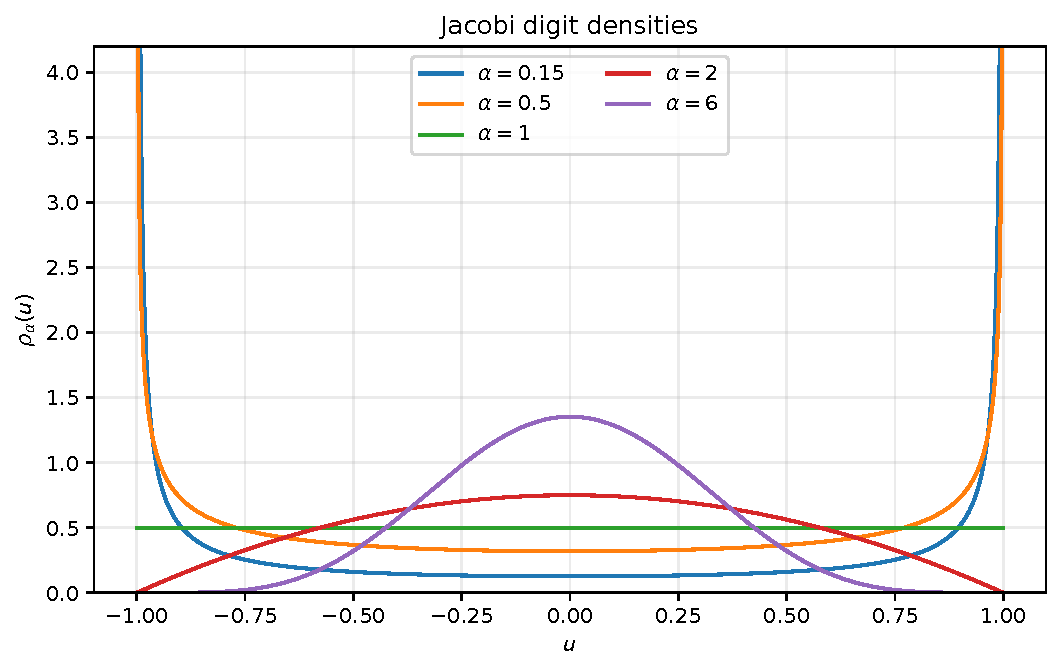
\includegraphics[width=0.82\textwidth]{jacobi_digit_densities.pdf}
\caption{The one-step Jacobi digit.  The limits \(\alpha\downarrow0\) and
\(\alpha\to\infty\) concentrate at the endpoints and at the origin,
respectively; standardization of the latter gives a Gaussian.}
\label{fig:digit-densities}
\end{figure}

\begin{theorem}[Fourier decay, smoothness, and positivity]
\label{thm:smoothness}
For each fixed \(q\in(0,1)\) and \(\alpha>0\),
\begin{equation}
 \log|\CharacteristicFunction{X_{q,\alpha}}(t)|
 \le -\frac{\alpha}{2L}(\log|t|)^2+O_{q,\alpha}(\log|t|)
 \qquad(|t|\to\infty)
 \label{eq:fourier-log-square-bound}
\end{equation}
away from its zeros, with the left side interpreted as \(-\infty\) at a
zero.  Consequently,
\[
 f_{q,\alpha}\in C_c^\infty(\RealNumbers),\qquad
 \SupportOperator(f_{q,\alpha})=[-1,1],
\]
and \(f_{q,\alpha}(x)>0\) for \(-1<x<1\).  Every derivative is flat at both
endpoints.
\end{theorem}

\begin{proof}
The large-argument Bessel estimate gives
\(|\Jcal_\nu(s)|\le C_{\alpha}|s|^{-\alpha}\) for \(|s|\ge1\), while a
characteristic function always has modulus at most one.  Put
\(T=\log(a|t|)\) and sum this estimate over the indices
\(0\le n\le T/L+O(1)\).  The logarithm of the product is at most
\[
 O(T)-\alpha\sum_{n\le T/L}(T-nL)
 =-\frac{\alpha}{2L}T^2+O(T),
\]
which is \eqref{eq:fourier-log-square-bound}.  The transform therefore decays
faster than every power, so Fourier inversion gives a \(C^\infty\) density.
The random series gives support contained in \([-1,1]\), while the support of
an infinite convolution is the closed Minkowski sum of the digit supports,
which is the whole interval.

For positivity, write \(X=aU+qX'\).  At an interior point \(x\), the intervals
\((-q,q)\) and \((x-a,x+a)\) have nonempty open intersection.  The law of
\(qX'\) assigns positive mass to every open subinterval of its support, and
the scaled digit kernel is positive on \((-a,a)\); their convolution is thus
positive at \(x\).  Compact support plus smoothness implies endpoint
flatness.
\end{proof}

The same argument in \(\RealNumbers^d\) proves that the spherical random-flight law in
\cref{thm:spherical-realization} has a \(C^\infty\) density on its annular or
ball support for every \(d\ge2\).

\begin{figure}[H]
\centering
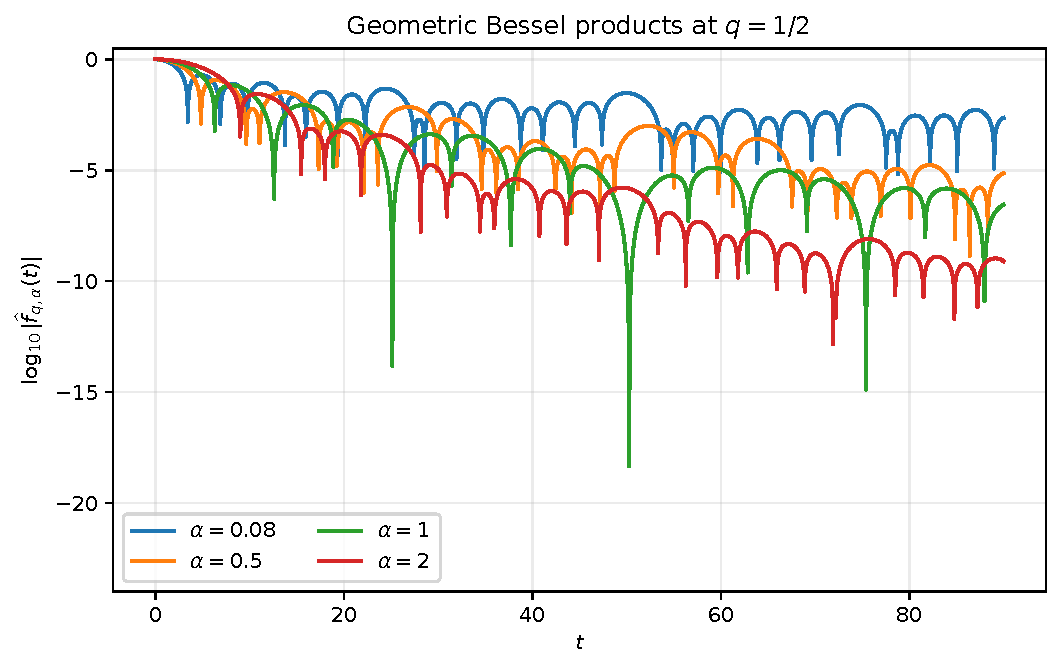
\includegraphics[width=0.82\textwidth]{geometric_bessel_products.pdf}
\caption{Logarithmic modulus of the geometric Bessel product at \(q=1/2\).
The zeros are inherited from geometrically rescaled Bessel zeros, while the
envelope obeys the quadratic logarithmic decay in
\eqref{eq:fourier-log-square-bound}.}
\label{fig:bessel-products}
\end{figure}

\begin{theorem}[Log-concavity above the Rvachev parameter]
\label{thm:log-concavity}
For every \(q\in(0,1)\) and \(\alpha\ge1\), the density
\(f_{q,\alpha}\) is log-concave on \(\RealNumbers\).  Hence it is unimodal and its
superlevel sets are intervals.
\end{theorem}

\begin{proof}
On \((-1,1)\),
\[
 \frac{d^2}{du^2}\log\rho_\alpha(u)
 =-2(\alpha-1)\frac{1+u^2}{(1-u^2)^2}\le0.
\]
Together with the convex support interval, this makes the extended digit
density log-concave.  Scaling and convolution preserve log-concavity by the
Pr\'ekopa--Leindler theorem \cite{Prekopa}.  Finite convolutions converge weakly to the
cascade, and the limiting smooth density inherits log-concavity.
\end{proof}

For \(0<\alpha<1\), the digit is U-shaped and log-concavity is no longer
automatic; numerical evidence in \cref{sec:numerics} suggests a nontrivial
shape phase diagram.

\subsection{A geometric \(q\)-Bessel coefficient array}

Expanding every \({}_0F_1\) factor gives an exact positive formula for all
even moments.

\begin{theorem}[Occupation-sum moment formula]
\label{thm:occupation-sum}
For \(N\ge0\),
\begin{equation}
 \frac{\Expectation X_{q,\alpha}^{2N}}{(2N)!}
 =\left(\frac{a^2}{4}\right)^N
 \sum_{\substack{k_0,k_1,\ldots\ge0\\k_0+k_1+\cdots=N}}
 \prod_{n=0}^{\infty}
 \frac{q^{2nk_n}}{k_n!\,\RisingFactorial{\alpha+1/2}{k_n}}.
 \label{eq:occupation-moment}
\end{equation}
Only finitely many \(k_n\) are nonzero in each summand.  Equivalently,
\begin{equation}
 \sum_{N\ge0}\frac{\Expectation X_{q,\alpha}^{2N}}{(2N)!}t^{2N}
 =\prod_{n\ge0}{}_0F_1\left(;\alpha+\frac12;
 \frac{a^2q^{2n}t^2}{4}\right).
 \label{eq:mgf-hypergeometric-product}
\end{equation}
\end{theorem}

\begin{proof}
Use the defining series for \({}_0F_1\) in the moment-generating version of
\eqref{eq:full-bessel-product}, multiply the absolutely convergent products,
and collect the total degree \(N=\sum k_n\).
\end{proof}

Formula \eqref{eq:occupation-moment} is not one of the standard Jackson or
Hahn--Exton \(q\)-Bessel functions; the \(q\)-dependence lies in a geometric
cascade of classical Bessel atoms.  It nevertheless supplies a natural
\(q\)-Bessel coefficient array tailored to the Fabius--Rvachev refinement
operator.

\section{Rayleigh cumulants, Bell moments, and Bernoulli specializations}
\label{sec:cumulants}

Let \(j_{\nu,1}<j_{\nu,2}<\cdots\) be the positive zeros of \(J_\nu\), and
define the Rayleigh sums
\begin{equation}
 R_m(\nu):=\sum_{k=1}^{\infty}j_{\nu,k}^{-2m}.
 \label{eq:rayleigh-definition}
\end{equation}
The classical Bessel product is
\begin{equation}
 \Jcal_\nu(z)=\prod_{k=1}^{\infty}
 \left(1-\frac{z^2}{j_{\nu,k}^2}\right).
 \label{eq:bessel-hadamard}
\end{equation}

\begin{lemma}[Rayleigh recurrence]
\label{lem:rayleigh-recurrence}
For \(\nu>-1\),
\begin{equation}
 R_1(\nu)=\frac1{4(\nu+1)},\qquad
 R_m(\nu)=\frac1{\nu+m}
 \sum_{r=1}^{m-1}R_r(\nu)R_{m-r}(\nu),\quad m\ge2.
 \label{eq:rayleigh-recurrence}
\end{equation}
\end{lemma}

\begin{proof}
The normalized Bessel function \(y=\Jcal_\nu\) satisfies
\(y''+(2\nu+1)y'/z+y=0\).  From \eqref{eq:bessel-hadamard},
\[
 w(z):=-\frac{y'(z)}{y(z)}=2\sum_{m\ge1}R_m(\nu)z^{2m-1}.
\]
The Bessel equation becomes the Riccati equation
\(w'=w^2-(2\nu+1)w/z+1\).  Comparing coefficients gives
\eqref{eq:rayleigh-recurrence}; this is Kishore's classical recurrence
\cite{Kishore1963,GuptaMuldoon2000}.
\end{proof}

\begin{theorem}[Rayleigh-factorized cumulants]
\label{thm:cumulants}
All odd cumulants of \(X_{q,\alpha}\) vanish, and
\begin{equation}
 \boxed{
 \kappa_{2m}(X_{q,\alpha})
 =(-1)^{m+1}\frac{(2m)!}{m}
 R_m\!\left(\alpha-\frac12\right)
 \frac{(1-q)^{2m}}{1-q^{2m}}.}
 \label{eq:master-cumulant}
\end{equation}
If \([s]_q=(1-q^s)/(1-q)\), the scale factor is
\begin{equation}
 \frac{(1-q)^{2m}}{1-q^{2m}}
 =\frac{(1-q)^{2m-1}}{[2m]_q}.
 \label{eq:q-integer-factor}
\end{equation}
Thus the atom geometry and the geometric scale separate exactly into a
Rayleigh factor and a \(q\)-integer factor.
\end{theorem}

\begin{proof}
Taking a logarithm in \eqref{eq:bessel-hadamard} gives, near zero,
\[
 \log\Jcal_\nu(t)=-\sum_{m\ge1}\frac{R_m(\nu)}m t^{2m}.
\]
Comparison with
\(\log\Expectation e^{itU}=\sum_r\kappa_r(U)(it)^r/r!\) yields
\(\kappa_{2m}(U)=(-1)^{m+1}(2m)!R_m/m\).  Cumulants add over independent
summands and scale by the corresponding power, so summing
\(a^{2m}q^{2mn}\) proves \eqref{eq:master-cumulant}.
\end{proof}

The first five nonzero digit cumulants, generated both from
\eqref{eq:rayleigh-recurrence} and independently from the symbolic
\({}_0F_1\) logarithm, are
\begin{align}
 \kappa_2(U_\alpha)&=\frac1{2\alpha+1},\label{eq:k2}\\
 \kappa_4(U_\alpha)&=-\frac6{(2\alpha+1)^2(2\alpha+3)},\label{eq:k4}\\
 \kappa_6(U_\alpha)&=\frac{240}
 {(2\alpha+1)^3(2\alpha+3)(2\alpha+5)},\label{eq:k6}\\
 \kappa_8(U_\alpha)&=-\frac{5040(10\alpha+17)}
 {(2\alpha+1)^4(2\alpha+3)^2(2\alpha+5)(2\alpha+7)},\label{eq:k8}\\
 \kappa_{10}(U_\alpha)&=\frac{725760(14\alpha+31)}
 {(2\alpha+1)^5(2\alpha+3)^2(2\alpha+5)(2\alpha+7)(2\alpha+9)}.
 \label{eq:k10}
\end{align}

\begin{corollary}[Bell-polynomial moments]
\label{cor:bell-moments}
Let \(B_n\) denote the complete exponential Bell polynomial.  Then
\begin{equation}
 \Expectation X_{q,\alpha}^n
 =B_n\bigl(0,\kappa_2,0,\kappa_4,\ldots,\kappa_n\bigr),
 \label{eq:bell-moments}
\end{equation}
with the cumulants from \eqref{eq:master-cumulant}.  Equivalently,
\begin{equation}
 \mu_n=\sum_{r=1}^{n}\binom{n-1}{r-1}\kappa_r\mu_{n-r},
 \qquad \mu_0=1.
 \label{eq:bell-recurrence}
\end{equation}
The distributional fixed point also gives the positive recurrence
\begin{equation}
 (1-q^{2N})\mu_{2N}
 =\sum_{r=1}^{N}\binom{2N}{2r}
 a^{2r}q^{2N-2r}
 \frac{\RisingFactorial{1/2}{r}}{\RisingFactorial{\alpha+1/2}{r}}
 \mu_{2N-2r}.
 \label{eq:positive-moment-recurrence}
\end{equation}
\end{corollary}

\begin{proof}
Equation \eqref{eq:bell-moments} is the standard moment--cumulant relation and
\eqref{eq:bell-recurrence} is its differentiated generating-function form.
Expanding \((aU+qX')^{2N}\), using symmetry and independence, and moving the
term with \(r=0\) to the left proves \eqref{eq:positive-moment-recurrence}.
\end{proof}

\subsection{Bernoulli numbers at two different boundaries}

At \(\alpha=1\), \(j_{1/2,k}=k\pi\), hence
\(R_m(1/2)=\zeta(2m)/\pi^{2m}\).  Euler's evaluation of \(\zeta(2m)\)
gives the familiar uniform-digit cumulants
\begin{equation}
 \kappa_{2m}(U_1)=\frac{2^{2m-1}B_{2m}}m,
 \qquad
 \kappa_{2m}(X_{q,1})
 =\frac{2^{2m-1}B_{2m}}m
 \frac{a^{2m}}{1-q^{2m}}.
 \label{eq:uniform-bernoulli-cumulants}
\end{equation}
This is an established repository specialization.

At the opposite limit \(\alpha\downarrow0\), the digit becomes a Rademacher
variable, whose cumulants are
\begin{equation}
 \kappa_{2m}(\varepsilon)
 =\frac{2^{2m}(2^{2m}-1)B_{2m}}{2m}.
 \label{eq:rademacher-cumulants}
\end{equation}
Thus Bernoulli numbers occur at both the uniform/Rvachev slice and the
Bernoulli-convolution boundary, but with different multipliers.  The Rayleigh
recurrence analytically interpolates between them.

\section{Fourier zeros, spectral zeta, and scale resonance}
\label{sec:spectral}

\subsection{Exact zero multiset and zeta factorization}

By \eqref{eq:full-bessel-product}, the positive Fourier-zero multiset is
\begin{equation}
 \Lambda_{q,\alpha}
 =\left\{\lambda_{n,k}:=
 \frac{j_{\nu,k}}{aq^n}:n\ge0,\ k\ge1\right\},
 \label{eq:zero-multiset}
\end{equation}
where coincidences are counted with multiplicity.

\begin{theorem}[Geometric Bessel spectral zeta]
\label{thm:spectral-zeta}
For \(\Re s>1\), let
\begin{equation}
 \zeta_\nu^{\mathrm B}(s)=\sum_{k\ge1}j_{\nu,k}^{-s},
 \qquad
 \Zcal_{q,\alpha}(s)=\sum_{n,k}\lambda_{n,k}^{-s}.
\end{equation}
Then
\begin{equation}
 \boxed{
 \Zcal_{q,\alpha}(s)
 =\frac{(1-q)^s}{1-q^s}\,
 \zeta_{\alpha-1/2}^{\mathrm B}(s)
 =\frac{(1-q)^{s-1}}{[s]_q}\,
 \zeta_{\alpha-1/2}^{\mathrm B}(s).}
 \label{eq:spectral-zeta-factorization}
\end{equation}
At the even positive integers,
\begin{equation}
 \kappa_{2m}(X_{q,\alpha})
 =(-1)^{m+1}\frac{(2m)!}{m}
 \Zcal_{q,\alpha}(2m).
 \label{eq:cumulant-zeta-identity}
\end{equation}
\end{theorem}

\begin{proof}
Insert \eqref{eq:zero-multiset}, separate the two absolutely convergent sums,
and evaluate \(\sum_{n\ge0}q^{ns}\).  Equation
\eqref{eq:cumulant-zeta-identity} is \eqref{eq:master-cumulant}.
\end{proof}

Under the standard meromorphic continuation of the Bessel zeta, the geometric
factor adds the lattice of possible poles
\begin{equation}
 \chi_\ell=\frac{2\pi i\ell}{L},\qquad \ell\in\IntegerNumbers,
 \label{eq:complex-dimensions}
\end{equation}
subject to cancellations by \(\zeta_\nu^{\mathrm B}\).  At a noncancelled
pole,
\begin{equation}
 \operatorname*{Res}_{s=\chi_\ell}\Zcal_{q,\alpha}(s)
 =\frac{a^{\chi_\ell}\zeta_\nu^{\mathrm B}(\chi_\ell)}{L}.
 \label{eq:complex-residue}
\end{equation}
These are the spectral counterpart of the log-periodic endpoint term proved
in \cref{thm:laplace-periodicity}.

\subsection{Resonance is exceptional but dense}

\begin{definition}[Resonant scales]
For fixed \(\nu>-1/2\), define
\begin{equation}
 \mathcal E_\nu
 :=\left\{
 \left(\frac{j_{\nu,k}}{j_{\nu,\ell}}\right)^{1/d}:
 1\le k<\ell,\ d\in\NaturalNumbers
 \right\}\subset(0,1).
 \label{eq:resonance-set}
\end{equation}
\end{definition}

\begin{theorem}[Countable-dense resonance dichotomy]
\label{thm:resonance}
The set \(\mathcal E_\nu\) is countable and dense in \((0,1)\).  If
\(q\notin\mathcal E_\nu\), every nonzero zero of
\(\CharacteristicFunction{X_{q,\alpha}}\) is simple.  If \(q\in\mathcal E_\nu\), at least one
zero has multiplicity at least two.  Hence simple zeros occur for Lebesgue
almost every \(q\), even though resonant \(q\)'s are dense.
\end{theorem}

\begin{proof}
Two factors share a positive zero precisely when
\[
 \frac{j_{\nu,\ell}}{aq^n}
 =\frac{j_{\nu,k}}{aq^{n+d}},
 \qquad d\ge1,
\]
which is equivalent to \(q^d=j_{\nu,k}/j_{\nu,\ell}\).  Bessel zeros are
simple, so absence of such an equality is equivalent to simplicity of the
full product zeros.  Countability is immediate.

For density it suffices to use \(d=1\).  McMahon's asymptotic formula \cite{Watson,DLMF}
\(j_{\nu,k}=\pi(k+\nu/2-1/4)+O(k^{-1})\) implies that, whenever
\(k_\ell/\ell\to r\in(0,1)\),
\(j_{\nu,k_\ell}/j_{\nu,\ell}\to r\).  Choosing
\(k_\ell=\Floor{r\ell}\) proves density.
\end{proof}

\begin{figure}[H]
\centering
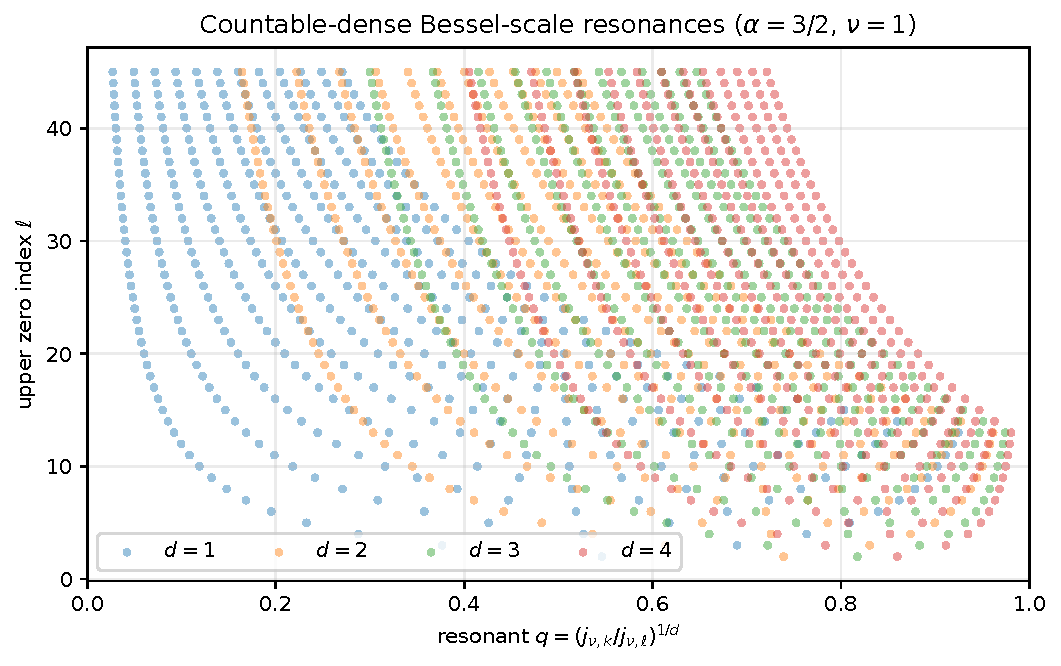
\includegraphics[width=0.82\textwidth]{bessel_resonance_cloud.pdf}
\caption{A finite sample of the countable-dense resonance set for
\(\alpha=3/2\), so \(\nu=1\).  The four point families correspond to scale
separations \(d=1,2,3,4\).}
\label{fig:resonance-cloud}
\end{figure}

The maximum gap among the ratios \(j_{1,k}/j_{1,\ell}\), augmented by zero and
one, decreases as follows:
\begin{center}
\begin{tabular}{rrrr}
\toprule
number of zeros & number of ratios & maximum gap & median gap\\
\midrule
10 & 45 & 0.11903523 & 0.01781670\\
20 & 190 & 0.06023619 & 0.00429132\\
40 & 780 & 0.03030307 & 0.00104959\\
80 & 3160 & 0.01519847 & 0.00026183\\
\bottomrule
\end{tabular}
\end{center}
This table is illustrative, not needed for the density proof.

\begin{corollary}[Sign from zero counting]
\label{cor:sign-count}
Away from its zeros,
\begin{equation}
 \Sign\CharacteristicFunction{X_{q,\alpha}}(t)
 =(-1)^{N_{q,\alpha}(|t|)},
 \label{eq:sign-zero-count}
\end{equation}
where \(N_{q,\alpha}(R)\) counts positive zeros at most \(R\), with
multiplicity.  At \(\alpha=1,q=1/2\), arithmetic coincidences among
\(j_{1/2,k}=k\pi\) reduce this parity to the dyadic Thue--Morse law already
proved in the repository.  For generic \(\alpha\), the ordering is governed
instead by Bessel-zero ratios.
\end{corollary}

\begin{theorem}[Universal zero-density law]
\label{thm:weyl-law}
Counting multiplicity,
\begin{equation}
 N_{q,\alpha}(R)=\frac{R}{\pi}+O_{q,\alpha}(\log R)
 \qquad(R\to\infty).
 \label{eq:zero-weyl}
\end{equation}
The leading density \(1/\pi\) is independent of both \(q\) and \(\alpha\).
\end{theorem}

\begin{proof}
The Bessel zero count satisfies \(N_\nu(x)=x/\pi+O_\nu(1)\).  Therefore
\[
 N_{q,\alpha}(R)=\sum_{n\ge0}N_\nu(aq^nR).
\]
Only \(O(\log R)\) summands are nonzero.  The main terms sum to
\[
 \frac{aR}{\pi}\sum_{n\ge0}q^n=\frac R\pi,
\]
and truncating this geometric sum where \(aq^nR\asymp1\) changes it by
\(O(1)\).  The bounded error in each active level contributes
\(O(\log R)\).
\end{proof}

For the sinc slice, the \(O(\log R)\) term contains digital sums.  For generic
Bessel zeros it becomes a quasidigital fluctuation generated by the orbit of
\(\log R\) modulo \(L\).  A smoothed counting function should admit a full
Fourier expansion from the residues \eqref{eq:complex-residue}; see
\cref{conj:spectral-fluctuation}.

\section{Higher-order Rvachev refinement equations}
\label{sec:higher-refinement}

The ordinary Rvachev law is distinguished by a uniform one-step kernel, whose
first distributional derivative consists of two endpoint delta masses.  For
integer \(\alpha=m\), the Jacobi kernel is a compact polynomial and the same
mechanism survives at order \(2m-1\).

Let
\begin{equation}
 k_{a,m}(x)=c_m a^{-(2m-1)}(a^2-x^2)^{m-1}_+,
 \qquad
 c_m=\frac{\Gamma(m+1/2)}{\sqrt\pi\,\Gamma(m)},
 \label{eq:integer-kernel}
\end{equation}
and \(g(x)=q^{-1}f_{q,m}(x/q)\).  The fixed point is \(f_{q,m}=k_{a,m}*g\).

\begin{theorem}[Finite higher-order refinement]
\label{thm:higher-refinement}
For every integer \(m\ge1\), in the classical sense on \(\RealNumbers\),
\begin{equation}
\boxed{
\begin{aligned}
 f_{q,m}^{(2m-1)}(x)
 &=(-1)^{m-1}c_ma^{-(2m-1)}
 \sum_{j=0}^{m-1}
 \frac{(2m-2-j)!(m-1)!}{(m-1-j)!j!}(2a)^j q^{-j-1}
 \\
 &\quad\times\left[
 (-1)^j f_{q,m}^{(j)}\left(\frac{x+a}{q}\right)
 -f_{q,m}^{(j)}\left(\frac{x-a}{q}\right)
 \right].
\end{aligned}}
 \label{eq:higher-refinement}
\end{equation}
Thus a compact polynomial digit of degree \(2m-2\) produces a finite
functional-differential equation of order \(2m-1\).
\end{theorem}

\begin{proof}
Put \(P(x)=(a^2-x^2)^{m-1}\) on \([-a,a]\) and zero outside.  Its
\((2m-1)\)-st distributional derivative is supported at the endpoints.  The
jump formula gives
\[
 D^{2m-1}P_+
 =\sum_{j=0}^{m-1}P^{(2m-2-j)}(a)
 \bigl((-1)^j\delta_{-a}^{(j)}-\delta_a^{(j)}\bigr).
\]
Only \(j\le m-1\) survives because \(P\) has a zero of order \(m-1\) at
each endpoint.  Leibniz' rule gives
\[
 P^{(2m-2-j)}(a)
 =(-1)^{m-1}
 \frac{(2m-2-j)!(m-1)!}{(m-1-j)!j!}(2a)^j.
\]
Convolution with \(g\), followed by
\(g^{(j)}(x)=q^{-j-1}f^{(j)}(x/q)\), proves
\eqref{eq:higher-refinement}.  The distributional identity is classical
because \(f\in C_c^\infty\).
\end{proof}

The first three equations are instructive.  For \(m=1\),
\begin{equation}
 f_{q,1}'(x)=\frac1{2aq}
 \left[f_{q,1}\left(\frac{x+a}{q}\right)
 -f_{q,1}\left(\frac{x-a}{q}\right)\right].
 \label{eq:m1-refinement}
\end{equation}
At \(q=a=1/2\), this is
\(\RvachevUp'(x)=2[\RvachevUp(2x+1)-\RvachevUp(2x-1)]\).
For \(m=2\),
\begin{equation}
\begin{aligned}
 f_{q,2}'''(x)
 &=-\frac{3}{2a^3q}
 \left[f_{q,2}\left(\frac{x+a}{q}\right)
 -f_{q,2}\left(\frac{x-a}{q}\right)\right]\\
 &\quad+\frac{3}{2a^2q^2}
 \left[f_{q,2}'\left(\frac{x+a}{q}\right)
 +f_{q,2}'\left(\frac{x-a}{q}\right)\right].
 \label{eq:m2-refinement}
\end{aligned}
\end{equation}
For \(m=3\),
\begin{equation}
\begin{aligned}
 f_{q,3}^{(5)}(x)
 &=\frac{45}{2a^5q}\,[f_+-f_-]
 -\frac{45}{2a^4q^2}\,[f_+'+f_-']
 +\frac{15}{2a^3q^3}\,[f_+''-f_-''],
 \label{eq:m3-refinement}
\end{aligned}
\end{equation}
where \(f_\pm^{(j)}=f_{q,3}^{(j)}((x\pm a)/q)\).

Equation \eqref{eq:higher-refinement} suggests replacing the scalar
Thue--Morse sign cocycle of \(m=1\) by a finite-dimensional jet cocycle for
\(m>1\).  This is made precise as a research problem in
\cref{conj:matrix-thue-morse}.

\section{Endpoint fractional pantographs and inverse asymptotics}
\label{sec:endpoint}

Let
\begin{equation}
 D_{q,\alpha}:=1-X_{q,\alpha}\in[0,2],
 \qquad
 G_{q,\alpha}(x):=\Probability(D_{q,\alpha}\le x).
 \label{eq:endpoint-def}
\end{equation}
Since \(V_\alpha=(1-U_\alpha)/2\sim\operatorname{Beta}(\alpha,\alpha)\),
\begin{equation}
 D_{q,\alpha}\ \overset d=\ 2aV_\alpha+qD'_{q,\alpha}.
 \label{eq:endpoint-fixed-point}
\end{equation}

\subsection{Exact Volterra equation}

\begin{proposition}[Endpoint Volterra--pantograph equation]
\label{prop:volterra}
For \(0<x<2a\),
\begin{equation}
 G(x)=\frac1{(2a)^\alpha B(\alpha,\alpha)}
 \int_0^x(x-y)^{\alpha-1}
 \left(1-\frac{x-y}{2a}\right)^{\alpha-1}
 G\left(\frac yq\right)\,dy.
 \label{eq:volterra-pantograph}
\end{equation}
\end{proposition}

\begin{proof}
Condition on \(2aV_\alpha=t\) in \eqref{eq:endpoint-fixed-point} and then
change variables from \(t\) to \(y=x-t\).
\end{proof}

For \(\beta>0\), write the left Riemann--Liouville integral as
\begin{equation}
 (\Iop^\beta h)(x)
 =\frac1{\Gamma(\beta)}\int_0^x(x-y)^{\beta-1}h(y)\,dy.
 \label{eq:RL-integral}
\end{equation}
Because \(G\) is flat at zero, the corresponding Riemann--Liouville derivative
\(\Dop^\alpha\) is an unambiguous left inverse of \(\Iop^\alpha\) here.

\begin{theorem}[Exact fractional endpoint equation]
\label{thm:fractional-pantograph}
For \(0<x<2a\),
\begin{equation}
\boxed{
 \Dop^\alpha G(x)
 =\frac{\Gamma(2\alpha)}{\Gamma(\alpha)(2a)^\alpha}
 \sum_{r=0}^{\infty}
 \frac{\RisingFactorial{\alpha}{r}\RisingFactorial{1-\alpha}{r}}
 {r!(2a)^r}
 \Iop^r\!\left[G\left(\frac{\cdot}{q}\right)\right](x).}
 \label{eq:fractional-endpoint-equation}
\end{equation}
The series converges locally absolutely for \(x<2a\).  If
\(\alpha=m\in\NaturalNumbers\), it terminates after \(r=m-1\).  For \(\alpha=1\),
\begin{equation}
 G'(x)=\frac1{2a}G(x/q),\qquad 0<x<2a.
 \label{eq:uniform-endpoint-G}
\end{equation}
\end{theorem}

\begin{proof}
Expand the second factor in \eqref{eq:volterra-pantograph}:
\[
 \left(1-\frac{x-y}{2a}\right)^{\alpha-1}
 =\sum_{r\ge0}\frac{\RisingFactorial{1-\alpha}{r}}{r!(2a)^r}(x-y)^r.
\]
On compact subintervals of \((0,2a)\), termwise integration is legitimate.
The integral in the \(r\)-th term is
\(\Gamma(\alpha+r)\Iop^{\alpha+r}[G(\cdot/q)]\).  Apply
\(\Dop^\alpha\), use
\(\Gamma(\alpha+r)=\Gamma(\alpha)\RisingFactorial{\alpha}{r}\), and simplify the beta
constant.  For convergence, \(\Iop^rh=O(x^r/r!)\), while the Pochhammer
coefficient grows only like \(r!/r\) up to a power; the resulting radius is
\(2a\).  If \(\alpha=m\), \(\RisingFactorial{1-m}{r}=0\) for \(r\ge m\).
\end{proof}

Under the common normalization
\(\Fab(x)=\RvachevUp(x-1)\) on \([0,1]\), symmetry gives
\(G_{1/2,1}'(x)=\Fab(x)\), while \eqref{eq:uniform-endpoint-G} gives
\(G_{1/2,1}'(x)=G_{1/2,1}(2x)\).  Hence
\begin{equation}
 \Fab(x)=G_{1/2,1}(2x),\qquad 0\le x\le\frac12.
 \label{eq:Fabius-G-relation}
\end{equation}
Thus \eqref{eq:fractional-endpoint-equation} is a genuine fractional-order
extension of the local Fabius equation, not merely an analogy.

\subsection{Endpoint Laplace product and periodic renormalization}

The beta Laplace transform is
\begin{equation}
 M_\alpha(s):=\Expectation e^{-sV_\alpha}
 ={}_1F_1(\alpha;2\alpha;-s).
 \label{eq:beta-laplace}
\end{equation}
Therefore
\begin{equation}
 \Expectation e^{-sD_{q,\alpha}}
 =\prod_{n\ge0}M_\alpha(2aq^ns).
 \label{eq:endpoint-laplace-product}
\end{equation}
Set \(C_\alpha=\Gamma(2\alpha)/\Gamma(\alpha)\) and
\(h_\alpha(y)=\log M_\alpha(y)\).  Standard Kummer asymptotics \cite{DLMF} give
\begin{equation}
 h_\alpha(y)=\log C_\alpha-\alpha\log y+O(y^{-1})
 \quad(y\to\infty),
 \qquad
 h_\alpha(y)=O(y)\quad(y\downarrow0).
 \label{eq:h-asymptotics}
\end{equation}

\begin{theorem}[Exact source of the log-periodic endpoint term]
\label{thm:laplace-periodicity}
Let
\[
 \Kcal_{\alpha,q}(z)=\sum_{n\ge0}h_\alpha(zq^n).
\]
There is a real-analytic, one-periodic function \(P_{\alpha,q}\) such that
\begin{equation}
 \Kcal_{\alpha,q}(z)
 =-\frac{\alpha}{2L}(\log z)^2
 +\left(\frac{\log C_\alpha}{L}-\frac\alpha2\right)\log z
 +P_{\alpha,q}\left(\frac{\log z}{L}\right)
 +O(z^{-1})
 \label{eq:laplace-periodic-asymptotic}
\end{equation}
as \(z\to\infty\), where the argument of \(P\) is taken modulo one.
An explicit convergent representation is obtained as follows.  For
\(0\le\theta<1\), put
\begin{align}
 P_{\alpha,q}(\theta)
 &=\sum_{m=-\infty}^{-1}h_\alpha(e^{L(m+\theta)})
 +\sum_{m=0}^{\infty}
 \bigl[h_\alpha(e^{L(m+\theta)})-\log C_\alpha
      +\alpha L(m+\theta)\bigr]
 \notag\\
 &\quad+\frac{\alpha L}{2}(\theta^2-\theta)
 +(\log C_\alpha)(1-\theta).
 \label{eq:periodic-profile-series}
\end{align}
\end{theorem}

\begin{proof}
Write \(\log z=L(N+\theta)\), where \(N=\Floor{\log z/L}\), and
reindex \(m=N-n\):
\[
 \Kcal(z)=\sum_{m=-\infty}^{N}h_\alpha(e^{L(m+\theta)}).
\]
For \(m\ge0\), add and subtract
\(\log C_\alpha-\alpha L(m+\theta)\).  The negative tail converges because
\(h_\alpha(e^{Lm})=O(e^{Lm})\); the corrected positive tail converges because
of the \(O(e^{-Lm})\) remainder in \eqref{eq:h-asymptotics}.  Summing the
subtracted arithmetic progression and replacing \(N\) by
\(\log z/L-\theta\) gives the quadratic and linear terms in
\eqref{eq:laplace-periodic-asymptotic}, plus precisely the last line of
\eqref{eq:periodic-profile-series}.  Reindexing proves one-periodicity.
For real analyticity, complexify \(\theta\).  The beta Laplace transform is
zero-free in a fixed relative neighborhood of the positive axis for sufficiently
small and sufficiently large arguments (by its Taylor and Kummer expansions),
and compactness handles the intervening annulus.  Hence the logarithms can be
chosen in a common strip \(|\Im\theta|<\eta\), where both tails converge
normally.  Their sum is holomorphic in that strip and therefore real analytic
on the real axis.  The omitted positive tail is
\(O(e^{-LN})=O(z^{-1})\).
\end{proof}

\begin{figure}[H]
\centering
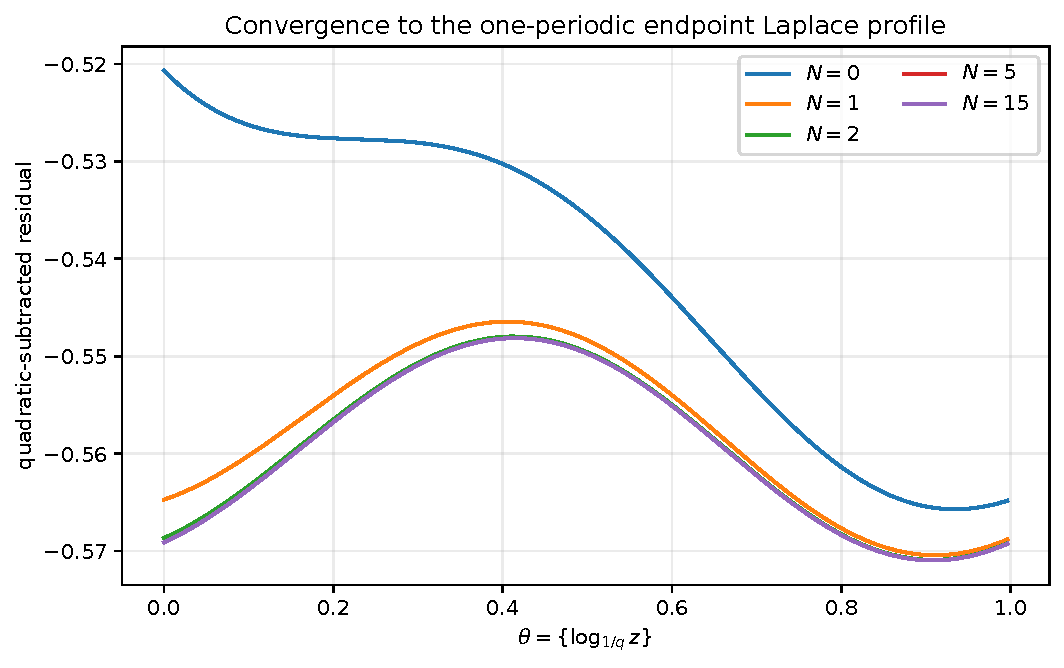
\includegraphics[width=0.82\textwidth]{endpoint_laplace_periodic_profile.pdf}
\caption{After subtraction of the quadratic and linear terms in
\eqref{eq:laplace-periodic-asymptotic}, successive logarithmic decades
converge rapidly to the same one-periodic profile.  The plotted parameters are
\(\alpha=1.3,q=0.1\).}
\label{fig:laplace-periodic}
\end{figure}

\subsection{Small balls and inverse quantiles}

\begin{theorem}[Endpoint log-square law]
\label{thm:small-ball}
As \(x\downarrow0\),
\begin{equation}
 \boxed{
 \lim_{x\downarrow0}
 \frac{\log G_{q,\alpha}(x)}{(\log(1/x))^2}
 =-\frac{\alpha}{2\log(1/q)}.}
 \label{eq:small-ball-leading}
\end{equation}
More quantitatively,
\begin{equation}
 \log G_{q,\alpha}(x)
 =-\frac{\alpha}{2L}(\log(1/x))^2
 +O_{q,\alpha}(\log(1/x)\log\log(1/x)).
 \label{eq:small-ball-error}
\end{equation}
\end{theorem}

\begin{proof}
Write \(D=\sum b_nV_n\), where \(b_n=2aq^n\).  Near zero, the beta CDF
satisfies \(c_1y^\alpha\le\Probability(V\le y)\le c_2y^\alpha\).

For an upper bound, choose \(N\) so that \(b_N\gtrsim x\).  The event
\(D\le x\) implies \(V_n\le x/b_n\) for \(0\le n\le N\).  Independence gives
\[
 \log G(x)\le\alpha\sum_{n=0}^{N}(\log x-\log b_n)+O(N).
\]
Since \(N=\log(1/x)/L+O(1)\), the arithmetic sum has leading term
\(-\alpha(\log(1/x))^2/(2L)\).

For a lower bound, choose \(N\) so the deterministic tail
\(\sum_{n>N}b_n=2q^{N+1}\le x/2\), and impose
\(b_nV_n\le x/[2(N+1)]\) for every \(n\le N\).  This event implies
\(D\le x\), and its logarithmic probability is the same arithmetic sum with
an additional \(-\alpha(N+1)\log(2N+2)+O(N)\).  The latter is
\(O(\log(1/x)\log\log(1/x))\), proving both claims.
\end{proof}

Let \(Q_{q,\alpha}(y)=G_{q,\alpha}^{-1}(y)\) be the lower endpoint quantile.

\begin{corollary}[Inverse endpoint scale]
\label{cor:inverse-quantile}
As \(y\downarrow0\),
\begin{equation}
 \boxed{
 \log\frac1{Q_{q,\alpha}(y)}
 \sim\sqrt{\frac{2\log(1/q)}{\alpha}\log\frac1y}.}
 \label{eq:inverse-quantile-leading}
\end{equation}
For the usual Fabius normalization,
\begin{equation}
 \Fab^{-1}(y)
 =\frac12\exp\left[-\sqrt{2\log2\,\log(1/y)}\,(1+o(1))\right].
 \label{eq:inverse-Fabius-leading}
\end{equation}
\end{corollary}

\begin{proof}
Monotonic inversion of \eqref{eq:small-ball-leading} gives
\eqref{eq:inverse-quantile-leading}.  Equation
\eqref{eq:Fabius-G-relation} implies
\(\Fab^{-1}(y)=Q_{1/2,1}(y)/2\) for small \(y\).
\end{proof}

\begin{conjecture}[Periodic Lambert-\(W_{-1}\) transseries]
\label{conj:lambert-transseries}
Let \(s_x\) be the positive saddle satisfying
\[
 \frac{d}{ds}\log\Expectation e^{-sD_{q,\alpha}}+x=0,
 \qquad T_x=\log(2as_x).
\]
Then
\begin{equation}
 T_x=-\Wm\!\left(-\frac{Lx}{2a\alpha}\right)+O(1),
 \label{eq:Lambert-leading-saddle}
\end{equation}
and the complete endpoint expansion is obtained by steepest descent from
\begin{equation}
 G(x)\sim
 \frac{\exp\{\Kcal_{\alpha,q}(2as_x)+s_xx\}}
 {s_x\sqrt{2\pi\,\Kcal_{\alpha,q}''(2as_x)(2a)^2}}
 \left(1+\sum_{r\ge1}\frac{c_r(\{T_x/L\})}{T_x^r}\right),
 \label{eq:conjectural-saddle-expansion}
\end{equation}
where every \(c_r\) is one-periodic and real analytic.  Reversion of this
series gives a complete inverse-quantile expansion.  At \(\alpha=1,q=1/2\),
it should coincide term by term with the repository's all-orders inverse
Fabius expansion after normalization changes.
\end{conjecture}

The leading Lambert relation (with the branch conventions of \cite{CorlessLambert}) follows formally by differentiating
\eqref{eq:laplace-periodic-asymptotic}: \(xs\sim\alpha T/L\), and hence
\(Te^{-T}\sim Lx/(2a\alpha)\).  The unresolved part is a uniform saddle-point
transfer retaining the periodic derivatives and controlling all remainder
terms.

\section{Boundary regimes: Bernoulli, Rvachev, and Gaussian}
\label{sec:boundary-regimes}

\subsection{The Bernoulli-convolution boundary \(\alpha\downarrow0\)}

Let \(\varepsilon_n\) be independent Rademacher variables and
\begin{equation}
 B_q=a\sum_{n\ge0}q^n\varepsilon_n.
 \label{eq:bernoulli-convolution}
\end{equation}
This is the normalized Bernoulli convolution with parameter \(q\); see, for context, \cite{PeresSolomyak,Hochman,Shmerkin}.

\begin{theorem}[Uniform Wasserstein desingularization rate]
\label{thm:W1-boundary}
For every \(q\in(0,1)\),
\begin{equation}
 W_1(\mu_{q,\alpha},\operatorname{Law}(B_q))
 \le 1-\frac{\Gamma(\alpha+1/2)}{\sqrt\pi\,\Gamma(\alpha+1)}
 =2\alpha\log2+O(\alpha^2)
 \label{eq:W1-bound}
\end{equation}
as \(\alpha\downarrow0\).  The bound is independent of \(q\).
Consequently, \(X_{q,\alpha}\Rightarrow B_q\) uniformly in the scale
parameter in the \(W_1\) sense.
\end{theorem}

\begin{proof}
Couple \(\varepsilon_n=\Sign(U_{\alpha,n})\).  By symmetry it is Rademacher,
and
\[
 \Expectation|X_{q,\alpha}-B_q|
 \le a\sum_{n\ge0}q^n\Expectation(1-|U_\alpha|)
 =1-\Expectation|U_\alpha|.
\]
Use \eqref{eq:digit-absolute-moment} with \(p=1\).  The expansion follows by
differentiating the logarithm of the gamma ratio at zero and using
\(\psi(1/2)-\psi(1)=-2\log2\).
\end{proof}

For every \(\alpha>0\), \cref{thm:smoothness} gives a positive
\(C_c^\infty\) density.  At \(\alpha=0\), however, the limit can be singular:
for \(q<1/2\) it is the separated Cantor-type Bernoulli measure.  Thus
\(\alpha\) is a genuine smooth desingularization parameter.  At the critical
value \(q=1/2\), the binary product identity
\begin{equation}
 \prod_{n=0}^{\infty}\cos(2^{-n-1}t)=\frac{\sin t}{t}
 \label{eq:cos-sinc-product}
\end{equation}
shows that the \(\alpha=0\) limit is uniform on \([-1,1]\), while
\(\alpha=1\) is the Rvachev \(\RvachevUp\) law.

\begin{figure}[H]
\centering
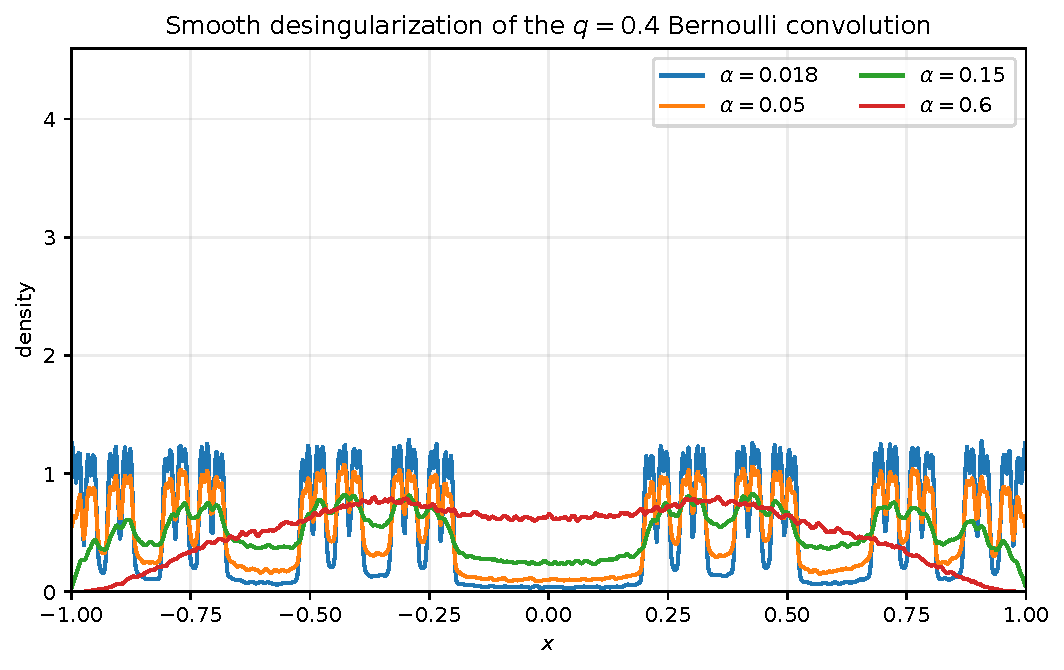
\includegraphics[width=0.82\textwidth]{bernoulli_desingularization_q_0p4.pdf}
\caption{For \(q=0.4<1/2\), small positive \(\alpha\) gives a smooth density
that increasingly resolves the gaps and peaks of the limiting Cantor-type
Bernoulli convolution.  The figure is a fixed-seed histogram and is used only
for qualitative shape evidence.}
\label{fig:bernoulli-desingularization}
\end{figure}

\begin{figure}[H]
\centering
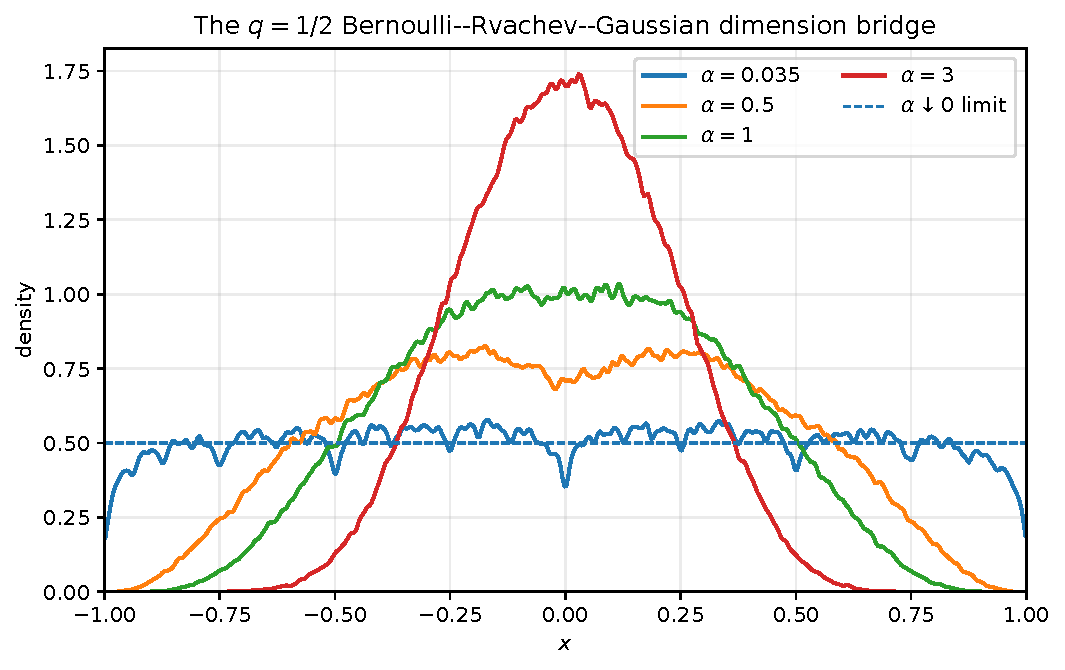
\includegraphics[width=0.82\textwidth]{cascade_density_bridge_q_half.pdf}
\caption{At \(q=1/2\), \(\alpha\downarrow0\) tends to the uniform density;
\(\alpha=1\) is the Rvachev law; increasing \(\alpha\) produces an
increasingly Gaussian central profile after the natural variance change.}
\label{fig:density-bridge}
\end{figure}

\subsection{Gaussianization as \(q\uparrow1\)}

Let \(Z_{q,\alpha}=X_{q,\alpha}/\sigma_{q,\alpha}\), with variance from
\eqref{eq:cascade-variance}.  The standardized cumulants factor as
\begin{equation}
 \lambda_{2m}(q,\alpha)
 :=\frac{\kappa_{2m}(X_{q,\alpha})}{\sigma_{q,\alpha}^{2m}}
 =\lambda_{2m}(U_\alpha)
 \frac{(1-q^2)^m}{1-q^{2m}}.
 \label{eq:standardized-cumulant-factor}
\end{equation}
In particular,
\begin{align}
 \lambda_4(q,\alpha)
 &=-\frac6{2\alpha+3}\frac{1-q^2}{1+q^2},
 \label{eq:lambda4}\\
 \lambda_6(q,\alpha)
 &=\frac{240}{(2\alpha+3)(2\alpha+5)}
 \frac{(1-q^2)^2}{1+q^2+q^4}.
 \label{eq:lambda6}
\end{align}

\begin{theorem}[Central limit and Berry--Esseen scale]
\label{thm:CLT-q}
For fixed \(\alpha>0\),
\begin{equation}
 Z_{q,\alpha}\Rightarrow N(0,1)\qquad(q\uparrow1).
 \label{eq:q-CLT}
\end{equation}
Moreover, with \(C_{\mathrm{BE}}\) any valid universal Berry--Esseen constant,
\begin{equation}
 d_{\mathrm K}(Z_{q,\alpha},N(0,1))
 \le C_{\mathrm{BE}}\,
 \rho_3(\alpha)\frac{(1-q^2)^{3/2}}{1-q^3},
 \label{eq:berry-esseen}
\end{equation}
where
\begin{equation}
 \rho_3(\alpha)
 =(2\alpha+1)^{3/2}
 \frac{\Gamma(\alpha+1/2)}{\sqrt\pi\,\Gamma(\alpha+2)}.
 \label{eq:rho3}
\end{equation}
The right side is \(O_\alpha(\sqrt{1-q})\).
\end{theorem}

\begin{proof}
Apply the Berry--Esseen theorem \cite{Petrov,BhattacharyaRao} to finite truncations of the independent weighted sum and
pass to the limit.  The ratio of the weighted third absolute moment to the
variance to the power \(3/2\) is
\[
 \frac{\sum a^3q^{3n}\Expectation|U|^3}
 {\left(\sum a^2q^{2n}\Variance U\right)^{3/2}}
 =\rho_3(\alpha)\frac{(1-q^2)^{3/2}}{1-q^3}.
\]
The asymptotic order follows by expansion at \(q=1\).
\end{proof}

\subsection{Gaussianization as \(\alpha\to\infty\)}

For fixed \(q\), \eqref{eq:standardized-cumulant-factor} and
\eqref{eq:k4}--\eqref{eq:k10} show
\begin{equation}
 \lambda_{2m}(q,\alpha)=O_{m,q}(\alpha^{1-m}),\qquad m\ge2.
 \label{eq:alpha-cumulant-decay}
\end{equation}
Moment convergence therefore gives a second Gaussian route.

\begin{theorem}[Two-parameter Gaussian corner]
\label{thm:two-parameter-gaussian}
If either \(q\uparrow1\) with \(\alpha\) bounded away from zero, or
\(\alpha\to\infty\) with \(q\) in a compact subset of \((0,1)\), then
\(Z_{q,\alpha}\Rightarrow N(0,1)\).  In particular, the conclusion holds
along every path with \((1-q)+\alpha^{-1}\to0\).  On bounded Fourier
intervals,
\begin{equation}
 \log\Expectation e^{itZ_{q,\alpha}}
 =-\frac{t^2}{2}+\frac{\lambda_4t^4}{24}+O(t^6\lambda_6+t^8\lambda_4^2).
 \label{eq:mod-gaussian}
\end{equation}
At the level of the first formal Edgeworth approximation, the density correction is
\begin{equation}
 \varphi(z)\left[1+\frac{\lambda_4}{24}H_4(z)\right],
 \qquad H_4(z)=z^4-6z^2+3.
 \label{eq:edgeworth}
\end{equation}
\end{theorem}

\begin{proof}
All fixed moments converge to the Gaussian moments by the cumulant formulas;
normal moment determinacy identifies the limit.  The logarithmic
characteristic-function expansion is the cumulant series, uniformly on
bounded \(t\)-sets when the parameters are sufficiently close to the
corner.  The displayed Edgeworth expression records the coefficient selected by the
cumulant expansion.  A uniform density remainder along a chosen two-parameter
path additionally requires a path-uniform Fourier-tail estimate; the
superpolynomial product bound supplies a natural route to such a refinement.
\end{proof}

\begin{figure}[H]
\centering
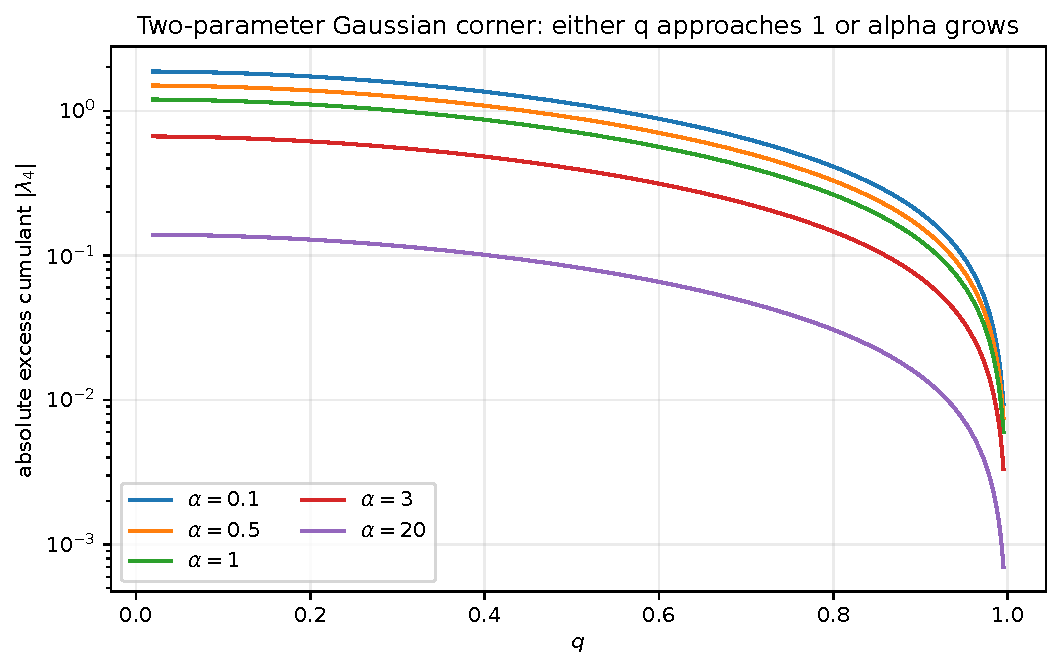
\includegraphics[width=0.82\textwidth]{two_parameter_gaussian_corner.pdf}
\caption{The exact magnitude of the excess fourth cumulant.  It vanishes by
either route: \(q\uparrow1\) or \(\alpha\to\infty\).}
\label{fig:gaussian-corner}
\end{figure}

\section{Jacobi--Gegenbauer to Hermite orthogonal flow}
\label{sec:orthogonal}

Let \(p_n^{(q,\alpha)}\) be the monic orthogonal polynomials of
\(\mu_{q,\alpha}\).  Symmetry gives
\begin{equation}
 p_{n+1}(x)=xp_n(x)-\beta_n(q,\alpha)p_{n-1}(x),
 \qquad \beta_n>0.
 \label{eq:monic-recurrence}
\end{equation}

\subsection{The two solvable edges}

\begin{theorem}[Jacobi edge and Hermite corner]
\label{thm:orthogonal-limits}
The family extends continuously to \(q=0\), where its measure is
\(\rho_\alpha(x)dx\), and
\begin{equation}
 \beta_n(0,\alpha)
 =\frac{n(n+2\alpha-2)}
 {4(n+\alpha-1/2)(n+\alpha-3/2)}.
 \label{eq:Gegenbauer-beta}
\end{equation}
This is the monic Gegenbauer/Jacobi recurrence, with the usual limiting
interpretation at \(\alpha=1/2,n=1\).  At \(\alpha=1\), it is the monic
Legendre recurrence.

After variance normalization, for every fixed \(n\),
\begin{equation}
 \frac{\beta_n(q,\alpha)}{\sigma_{q,\alpha}^2}\longrightarrow n
 \label{eq:Hermite-beta-limit}
\end{equation}
whenever \((q,\alpha)\) approaches the Gaussian corner of
\cref{thm:two-parameter-gaussian}.  Hence the standardized monic polynomials
converge coefficientwise to the probabilists' Hermite polynomials.
\end{theorem}

\begin{proof}
At \(q=0\), \(X_{0,\alpha}=U_\alpha\), whose weight is the Gegenbauer weight
with parameter \(\lambda=\alpha-1/2\).  Converting the standard Gegenbauer
recurrence \cite{Szego} to monic form gives \eqref{eq:Gegenbauer-beta}.  At the Gaussian
corner, every finite moment matrix converges to its Gaussian counterpart.
Hankel determinant formulas for the monic recurrence coefficients are
continuous because the limiting determinants are positive, and the Gaussian
coefficients are \(n\).
\end{proof}

This is a two-parameter extension of the Legendre--Hermite bridge: \(q\)
controls the number of effective geometric digits, while \(\alpha\) controls
the spherical/Jacobi shape of each digit.

\subsection{Exact first coefficients}

Put \(v=\sigma_{q,\alpha}^2\).  For any centered symmetric law with
standardized cumulants \(\lambda_4,\lambda_6\), Gram--Schmidt gives
\begin{align}
 \beta_1&=v,\label{eq:beta1}\\
 \frac{\beta_2}{v}&=2+\lambda_4,
 \label{eq:beta2-general}\\
 \frac{\beta_3}{v}
 &=\frac{6+9\lambda_4+\lambda_6-\lambda_4^2}{2+\lambda_4}.
 \label{eq:beta3-general}
\end{align}
Therefore
\begin{equation}
 \boxed{
 \frac{\beta_2(q,\alpha)}v
 =2-\frac6{2\alpha+3}\frac{1-q^2}{1+q^2}.}
 \label{eq:beta2-exact}
\end{equation}

\begin{proposition}[Monotonicity of the second coefficient]
\label{prop:beta2-monotone}
The normalized coefficient \(\beta_2/v\) is strictly increasing in both
\(q\) and \(\alpha\), from its Jacobi value at \(q=0\) to the Hermite value
2 at \(q=1\).
\end{proposition}

\begin{proof}
Differentiate the explicit expression \eqref{eq:beta2-exact}.
\end{proof}

\begin{figure}[H]
\centering
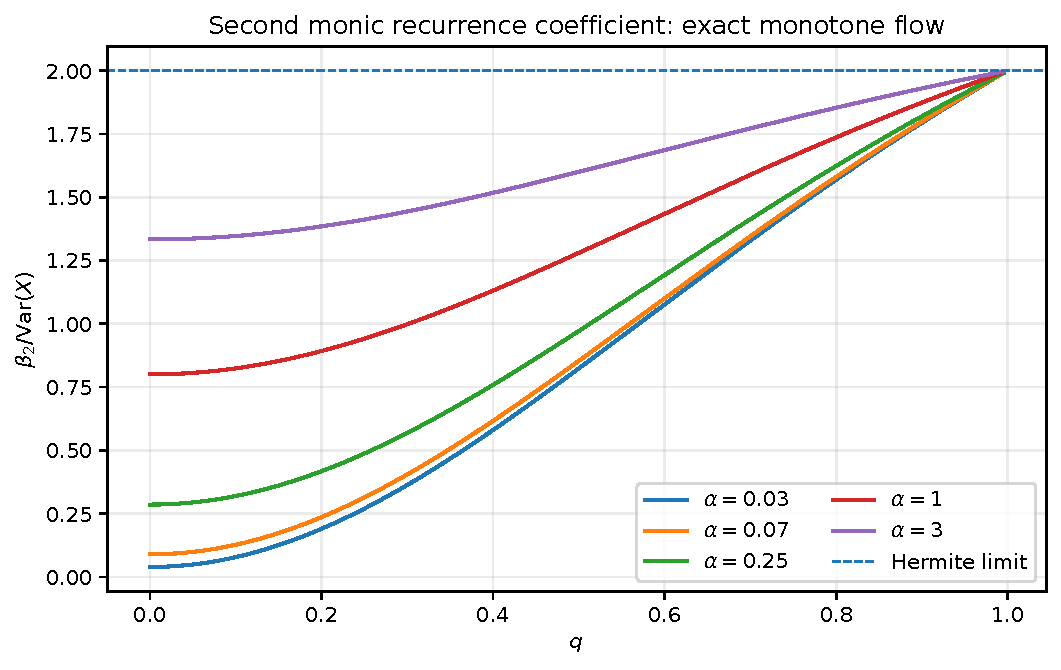
\includegraphics[width=0.82\textwidth]{orthogonal_beta2_flow.pdf}
\caption{The exact monotone Jacobi-to-Hermite flow of the second normalized
monic recurrence coefficient.}
\label{fig:beta2-flow}
\end{figure}

The third coefficient has a more surprising geometry.  Set
\begin{equation}
 A=2\alpha+3>3,
 \qquad x=q^2\in(0,1).
\end{equation}
Substitution of \eqref{eq:lambda4}--\eqref{eq:lambda6} into
\eqref{eq:beta3-general} and symbolic differentiation gives
\begin{equation}
 \frac{d}{dx}\left(\frac{\beta_3}{v}\right)
 =\frac{36P_A(x)}
 {A(A+2)(1+x)^2(1+x+x^2)^2(Ax+A+3x-3)^2},
 \label{eq:beta3-derivative}
\end{equation}
where
\begin{align}
 P_A(x)
 &=A^3(x^6+4x^5+8x^4+10x^3+8x^2+4x+1)\notag\\
 &\quad+A^2(10x^6+44x^5+62x^4+20x^3-30x^2-28x-6)\notag\\
 &\quad+A(3x^6+32x^5-18x^4-74x^3-2x^2+48x+11)\notag\\
 &\quad-6x^6+12x^3-6.
 \label{eq:PA-polynomial}
\end{align}
The denominator in \eqref{eq:beta3-derivative} is positive.  At the endpoints,
\[
 P_A(0)=(A-1)(A-2)(A-3)>0,
 \qquad P_A(1)=36A^2(A+2)>0.
\]
Thus any nonmonotonicity must be a genuine interior positive--negative--positive
turning pattern.

\begin{experiment}[Third-coefficient phase]
\label{exp:beta3-phase}
The included minimization and resultant computation find a tangency at
\begin{equation}
 \alpha_3^*=0.066515108060995\ldots,
 \quad
 q_*=0.319296212569559\ldots,
 \quad
 x_*=q_*^2=0.101950071361265\ldots.
 \label{eq:alpha3-star}
\end{equation}
For \(0<\alpha<\alpha_3^*\), \(P_A\) is negative on an interior interval;
for sampled \(\alpha>\alpha_3^*\), it is nonnegative on \([0,1]\).  The
candidate \(A_*=2\alpha_3^*+3\) is a real root of the degree-18 resultant
factor listed in \cref{app:beta3-polynomial}.
\end{experiment}

\begin{conjecture}[Sharp \(\beta_3\) monotonicity threshold]
\label{conj:beta3-threshold}
There is a unique threshold \(\alpha_3^*\) given by
\eqref{eq:alpha3-star} such that:
\begin{enumerate}[label=(\roman*)]
 \item if \(\alpha\ge\alpha_3^*\), then \(\beta_3/v\) is strictly increasing
       in \(q\in(0,1)\), except for the single horizontal tangency at equality;
 \item if \(0<\alpha<\alpha_3^*\), then \(\beta_3/v\) has one local maximum
       and one local minimum.
\end{enumerate}
A Sturm-sequence or cylindrical algebraic decomposition proof should be
feasible because the problem has been reduced to positivity of the explicit
bivariate polynomial \eqref{eq:PA-polynomial} on a rectangle.
\end{conjecture}

\begin{figure}[H]
\centering
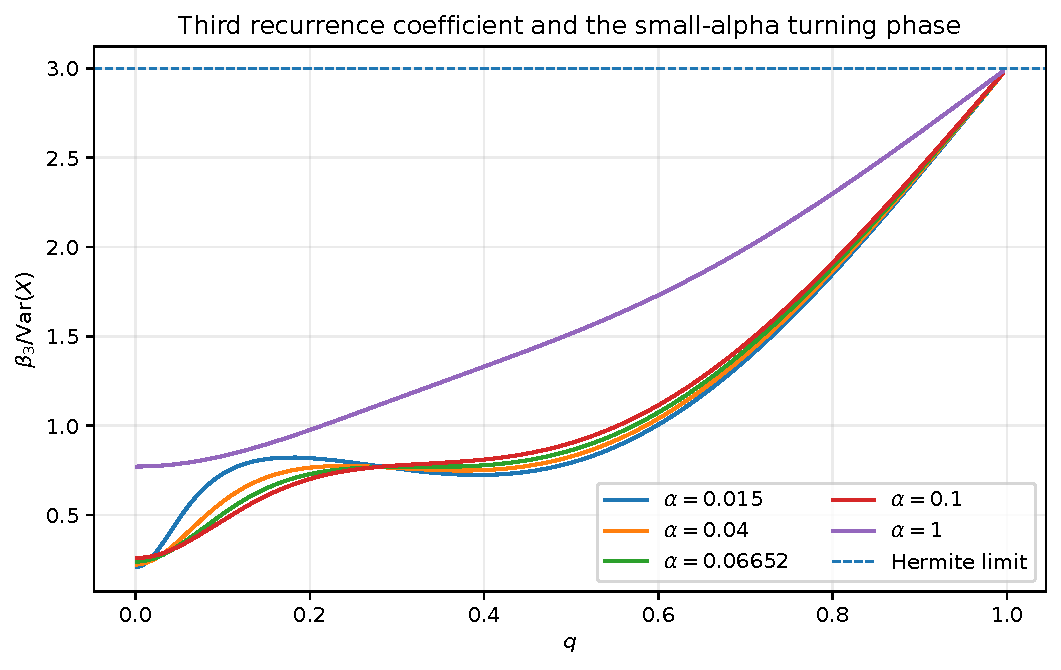
\includegraphics[width=0.82\textwidth]{orthogonal_beta3_flow.pdf}
\caption{The third coefficient.  Very small \(\alpha\) produces a local
maximum and minimum before the Hermite limit; the turning points merge at the
observed threshold.}
\label{fig:beta3-flow}
\end{figure}

\begin{figure}[H]
\centering
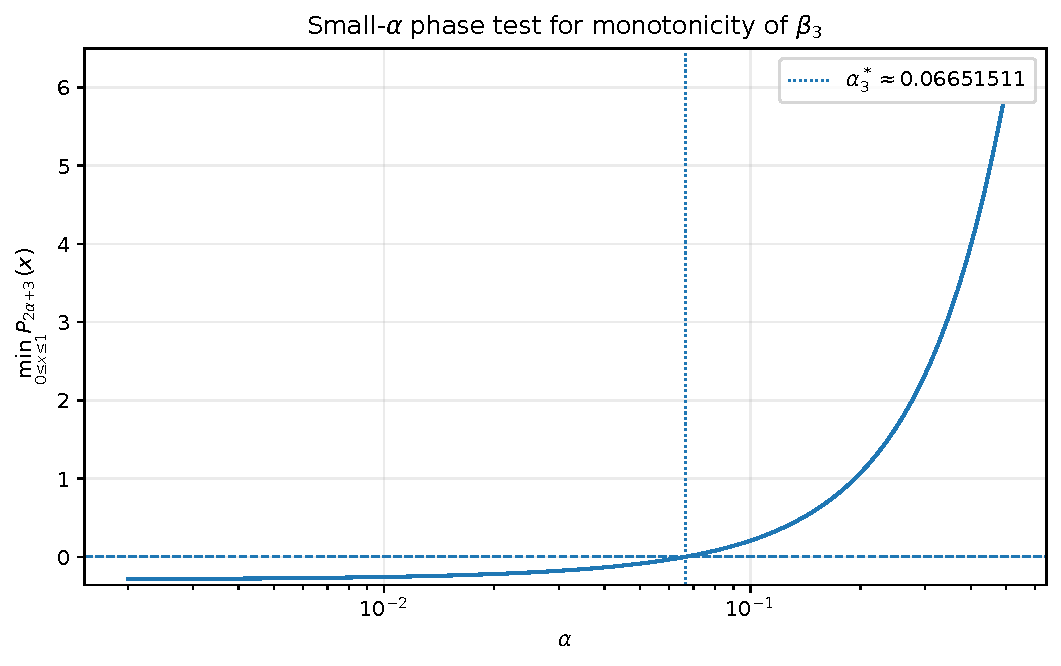
\includegraphics[width=0.82\textwidth]{beta3_monotonicity_phase.pdf}
\caption{Minimum of the exact derivative-controlling polynomial
\(P_{2\alpha+3}\) over \(0\le q^2\le1\).  The zero crossing identifies the
candidate threshold \(\alpha_3^*\).}
\label{fig:beta3-phase}
\end{figure}

\begin{conjecture}[Higher recurrence phase hierarchy]
\label{conj:higher-beta-phase}
For each \(n\ge3\), the normalized coefficient \(\beta_n/v\) has a finite
collection of critical \(\alpha\)-values at which its \(q\)-flow changes
turning topology.  These values are algebraic, obtained by eliminating
\(q^2\) from the numerator of \(\partial_q(\beta_n/v)\) and its derivative.
The sequence of largest thresholds tends to zero as \(n\to\infty\).
\end{conjecture}

The last assertion is deliberately speculative; it is motivated by the idea
that high-degree orthogonal polynomials resolve the increasingly fine
Bernoulli-like structure near \(\alpha=0\).

\section{Small-\(q\) and large-\(q\) expansions}
\label{sec:q-expansions}

The new family also provides controlled local expansions in the scale
parameter.  Write \(\phi_\alpha(t)=\Jcal_\nu(t)\).

\begin{proposition}[Expansion at \(q=0\)]
\label{prop:q0-expansion}
Uniformly for \(t\) in compact sets,
\begin{equation}
 \CharacteristicFunction{X_{q,\alpha}}(t)
 =\phi_\alpha(t)-qt\phi_\alpha'(t)
 +q^2\left[
 \frac{t^2}{2}\phi_\alpha''(t)
 -\frac{t^2}{2(2\alpha+1)}\phi_\alpha(t)
 \right]+O(q^3).
 \label{eq:q0-CF-expansion}
\end{equation}
Thus the first perturbation differentiates the Jacobi characteristic
function, while the second term contains the variance of the newly activated
second digit.
\end{proposition}

\begin{proof}
In \eqref{eq:full-bessel-product}, expand the first factor
\(\phi_\alpha((1-q)t)\) to second order.  The second factor has argument
\((1-q)qt=qt+O(q^2)\) and equals
\(1-q^2t^2/[2(2\alpha+1)]+O(q^3)\).  All remaining factors contribute
\(1+O(q^4)\).
\end{proof}

At \(q=1-\varepsilon\), the standardized cumulant factor satisfies
\begin{equation}
 \frac{(1-q^2)^m}{1-q^{2m}}
 =\frac{2^{m-1}}m\varepsilon^{m-1}
 \left(1+\frac{m-1}{2}\varepsilon+O(\varepsilon^2)\right).
 \label{eq:q1-cumulant-expansion}
\end{equation}
Together with the Rayleigh recurrence, this generates the complete formal
Edgeworth expansion to arbitrary order.  The coefficients are rational in
\(\alpha\), \(q\)-integer factors, and complete Bell polynomials; no Bessel
zero computation is required.

At large \(\alpha\), for example,
\begin{align}
 \lambda_4(U_\alpha)&=-\frac3\alpha+O(\alpha^{-2}),\notag\\
 \lambda_6(U_\alpha)&=\frac{60}{\alpha^2}+O(\alpha^{-3}),\notag\\
 \lambda_8(U_\alpha)&=-\frac{3150}{\alpha^3}+O(\alpha^{-4}).
 \label{eq:large-alpha-cumulants}
\end{align}
These can be inserted into \eqref{eq:standardized-cumulant-factor} to obtain a
two-variable asymptotic expansion near the Gaussian corner.

\section{Numerical experiments and reproducibility}
\label{sec:numerics}

The archive contains \path{experiments.py}, \texttt{requirements.txt}, all
CSV outputs, and both PDF and PNG versions of every figure.  The program uses:
\begin{itemize}
 \item exact Rayleigh recurrences and Bell recurrences for cumulants and
       moments;
 \item 80-digit Hankel determinants for monic recurrence coefficients;
 \item corrected finite Bessel-zero sums as an independent check;
 \item fixed-seed Monte Carlo only for density visualization and a separate
       moment sanity check; and
 \item direct summation of the beta Laplace product to verify the periodic
       renormalization in \cref{thm:laplace-periodicity}.
\end{itemize}
The final run used seed 20260830, 320,000 samples per density curve, and
600,000 samples per moment-validation parameter pair.

\subsection{Validation results}

The corrected sums of 240 Bessel zeros agree with the Rayleigh recurrence
through \(R_5\) to a worst relative error of
\(1.10\times10^{-8}\).  Across the deliberately difficult parameter pairs
listed below, empirical even moments through order eight agree with the exact
Bell moments to a worst relative error below \(5.3\times10^{-3}\).

\begin{table}[H]
\centering
\small
\begin{tabular}{cccccc}
\toprule
\(\alpha\) & \(q\) & order & exact moment & empirical moment & relative error\\
\midrule
0.08 & 0.4 & 8 & 0.12213418 & 0.12200004 & $1.0983\times10^{-3}$\\
0.5 & 0.5 & 8 & 0.01426675 & 0.01424493 & $1.5294\times10^{-3}$\\
1.0 & 0.5 & 8 & 0.00408246 & 0.00410216 & $4.8254\times10^{-3}$\\
3.0 & 0.8 & 8 & $5.0084050\times10^{-6}$ & $5.0025652\times10^{-6}$ & $1.1660\times10^{-3}$\\
\bottomrule
\end{tabular}
\caption{Representative independent Monte Carlo checks.  Exact full-precision
values and actual empirical values are in
\protect\nolinkurl{data/moment_monte_carlo_validation.csv}.}
\label{tab:moment-validation}
\end{table}

No theorem in the report depends on Monte Carlo.  The numerical layer is used
to discover the orthogonal phase, visualize the singular boundary, and catch
algebraic or normalization errors.

\subsection{Interpretation of the density figures}

\Cref{fig:bernoulli-desingularization} shows that the limit
\(\alpha\downarrow0\) is not uniform in pointwise topology when \(q<1/2\):
the densities remain smooth for every positive \(\alpha\) but develop
increasingly fine peaks separated by valleys.  This makes the Wasserstein
bound \eqref{eq:W1-bound} a natural metric statement; uniform density bounds
cannot hold.

At \(q=1/2\), \cref{fig:density-bridge} displays the dimension ladder
\[
 S^0\ \longrightarrow\ S^1\ \longrightarrow\ S^2
 \ \longrightarrow\ \text{high-dimensional spheres},
\]
projected through the same geometric random flight.  The Rvachev law is not an
isolated object in this picture: it is the \(d=3\) coordinate of a continuum
of analytically continued spherical dimensions \(d=2\alpha+1\).

\section{Conjectures and frontier research program}
\label{sec:future}

\subsection{Arithmetic and spectral questions}

\begin{conjecture}[Algebraic nonresonance]
\label{conj:algebraic-nonresonance}
Let \(\alpha>0\) be rational with \(\alpha\ne1\).  For algebraic
\(q\in(0,1)\), no equality
\[
 q^d=\frac{j_{\alpha-1/2,k}}{j_{\alpha-1/2,\ell}}
\]
occurs, except for explicitly classifiable half-integer Bessel orders with
trigonometric reductions.  Equivalently, the Fourier zeros are simple at
algebraic scales outside a finite list of elementary cases.
\end{conjecture}

Even proving irrationality of individual ratios of Bessel zeros is difficult,
so this is a long-range target.  A weaker first step is to establish
nonresonance for almost every \(\alpha\) at a fixed algebraic \(q\), using
analytic dependence of Bessel zeros on order.

\begin{conjecture}[Smoothed spectral fluctuation]
\label{conj:spectral-fluctuation}
A first Riesz mean of \(N_{q,\alpha}(R)\) has an expansion consisting of a
universal linear term, an \(\alpha\)-dependent logarithmic term, and a bounded
one-periodic function of \(\log R/L\).  Its Fourier coefficients are residues
of \(\Gamma(s)\Zcal_{q,\alpha}(s)\) at \(s=2\pi i\ell/L\).
\end{conjecture}

The unsmoothed sinc case contains binary digit sums, so smoothing is essential
if one wants a bounded periodic remainder.

\subsection{A matrix-valued Thue--Morse extension}

\begin{conjecture}[Jet cocycle and matrix automaticity]
\label{conj:matrix-thue-morse}
For integer \(m\ge2\) and reciprocal-integer scales \(q=1/b\), repeated use of
\eqref{eq:higher-refinement} can be organized as a finite-dimensional linear
cocycle on a jet vector of \(f_{q,m}\).  The branch matrices are indexed by
base-\(b\) digits.  At \(m=1,b=2\), their one-dimensional sign quotient is the
Thue--Morse sequence; at \(m>1\), matrix products give a \(b\)-regular
sequence controlling derivative signs and dyadic/radix rational values.
\end{conjecture}

A practical route is to choose the minimal jet closed under the two affine
branches in \eqref{eq:higher-refinement}, compute its semigroup, and ask
whether it admits a triangular or representation-theoretic reduction.

\subsection{Shape transition below \(\alpha=1\)}

\begin{conjecture}[Unimodality and log-concavity curves]
\label{conj:shape-curve}
There are critical curves \(q_{\mathrm{uni}}(\alpha)\) and
\(q_{\mathrm{lc}}(\alpha)\) on \(0<\alpha<1\) such that the cascade is,
respectively, unimodal and log-concave above the curves.  They satisfy
\[
 q_{\mathrm{lc}}(\alpha)\ge q_{\mathrm{uni}}(\alpha),
 \qquad
 \lim_{\alpha\uparrow1}q_{\mathrm{lc}}(\alpha)=0,
\]
and exhibit singular behavior as \(\alpha\downarrow0\) reflecting the
Bernoulli-convolution phase at \(q=1/2\).
\end{conjecture}

The Fourier product gives a direct numerical test through high-accuracy
inversion, while total positivity or variation-diminishing convolution may
supply proofs in part of the parameter plane.

\subsection{Endpoint and inverse problems}

The most immediate analytic problem is to prove
\cref{conj:lambert-transseries}.  The explicit periodic function
\eqref{eq:periodic-profile-series} removes one major ambiguity: periodic
coefficients are not fitted numerically but are convergent analytic sums.  A
complete solution should proceed through a uniform saddle theorem for
geometrically self-similar Laplace products, followed by transseries reversion
for \(Q_{q,\alpha}\).

Further questions include:
\begin{enumerate}[label=(\alph*)]
 \item determining how the fractional order \(\alpha\) enters the first
       logarithmic and \(\log\log\) corrections to
       \eqref{eq:inverse-quantile-leading};
 \item proving differentiability of the periodic profile with respect to both
       \(q\) and \(\alpha\), including limits at integer \(\alpha\);
 \item finding Stokes phenomena in the complex endpoint plane; and
 \item matching the \(\alpha\downarrow0\) endpoint expansion to large
       deviations of Bernoulli convolutions.
\end{enumerate}

\subsection{Orthogonal and interpolation questions}

The exact moment recurrence \eqref{eq:positive-moment-recurrence} makes the
Hankel determinants amenable to symbolic computation.  Promising targets are:
\begin{enumerate}[label=(\alph*)]
 \item a Sturm/CAD proof of \cref{conj:beta3-threshold};
 \item exact resultant phase diagrams for \(\beta_4,\beta_5\), followed by
       asymptotics in \(n\);
 \item Christoffel-function estimates uniform in the Jacobi--Hermite corner;
 \item geometric-comb interpolation in the basis
       \(p_n^{(q,\alpha)}\), comparing Lebesgue constants with the existing
       Legendre and native-\(\RvachevUp\) constructions; and
 \item a double-scaling universality regime in which
       \(n(1-q)\) and \(n/\alpha\) remain finite, potentially producing new
       transition kernels between Jacobi and Hermite asymptotics.
\end{enumerate}

\subsection{Vector random-flight questions}

The vector law \eqref{eq:vector-cascade} opens a separate geometric frontier.
At \(q<1/2\), its support has a flat inner boundary as well as a flat outer
boundary.  One can ask for coupled asymptotic expansions at both radii,
including the critical coalescence at \(q=1/2\).  Spherical harmonics should
diagonalize angular modes of the refinement operator, with Gegenbauer
polynomials governing coordinate projections.  This may produce a natural
multidimensional analogue of Rvachev atomic functions on balls and annuli.

\subsection{Formalization plan}

A staged Lean formalization can avoid measure-theoretic obstacles at first:
\begin{enumerate}[label=\arabic*.]
 \item formalize the rational Rayleigh recurrence and generate
       \eqref{eq:k2}--\eqref{eq:k10};
 \item formalize the algebraic cumulant scaling and Bell recurrence;
 \item prove the moment fixed-point recurrence
       \eqref{eq:positive-moment-recurrence};
 \item verify the exact \(\beta_2\) and \(\beta_3\) formulas by polynomial
       normalization;
 \item use a certified real-algebraic package for the
       \(P_A(x)\) positivity problem; and only then
 \item add probability measures, infinite convolutions, and distributional
       derivatives for the analytic theorems.
\end{enumerate}
The finite algebraic core is already well suited to exact computation and
would provide reusable infrastructure for the repository's existing
Bernoulli--Bell and orthogonal-polynomial developments.

\section{Conclusion}

Changing the scale parameter alone preserves the uniform digit and therefore
preserves the sinc atom.  Changing the digit to the Jacobi family exposes a
larger structure:
\[
 \boxed{\begin{gathered}
 \text{spherical geometry}
 \longleftrightarrow
 \text{Bessel zeros}
 \longleftrightarrow
 \text{Rayleigh cumulants}\\
 \longleftrightarrow
 \text{Jacobi orthogonality}
 \longleftrightarrow
 \text{fractional endpoint order}
 \end{gathered}}
\]
The Rvachev law sits at the particularly symmetric point \(d=3\),
\(\alpha=1\), while the Bernoulli convolution is the boundary \(d=1\),
\(\alpha=0\), and Hermite behavior appears at high dimension or high digit
density.  The same geometric series produces a \(q\)-integer spectral factor,
a dense resonance set, and log-periodic endpoint corrections.

The most robust new results are the exact formulas: the Bessel product,
Rayleigh cumulants, spectral-zeta factorization, higher-order refinement, and
fractional pantograph.  They are independent of numerical evidence and reduce
at \(\alpha=1\) to known repository formulas.  The numerics then reveal a
less expected phenomenon: orthogonal recurrence coefficients remember the
near-Bernoulli microstructure, producing a genuine turning phase long before
the density ceases to be smooth.  That phase, the complete Lambert expansion,
and the matrix Thue--Morse cocycle form a coherent next research program.

\appendix

\section{The resultant polynomial for the \(\beta_3\) phase}
\label{app:beta3-polynomial}

Eliminating \(x\) from \(P_A(x)=0\) and \(\partial_xP_A(x)=0\) produces several
extraneous or boundary factors and the following degree-18 factor:
\begin{align*}
 Q(A)={}&27A^{18}+324A^{17}-5670A^{16}-58320A^{15}
 +2599461A^{14}+23888916A^{13}\\
 &-213002432A^{12}-1553944800A^{11}+10096215141A^{10}
 +40741963244A^9\\
 &-197857358766A^8-118077559920A^7+579333364587A^6
 +348162442236A^5\\
 &-247263068556A^4-54019599840A^3+57183051600A^2
 -12550510656A+918330048.
\end{align*}
It has one real root greater than three,
\[
 A_*=3.133030216121990\ldots,
 \qquad \alpha_*=(A_*-3)/2.
\]
The other real roots are negative.  This algebraic isolation strongly
supports \cref{conj:beta3-threshold}; a complete proof must additionally
certify the sign of \(P_A\) over the two parameter cells separated by the
tangency.

\section{A direct formula for the periodic profile}

For reference, the proof of \cref{thm:laplace-periodicity} gives a numerically
stable algorithm.  Given \(\theta\in[0,1)\), sum the negative-index part of
\eqref{eq:periodic-profile-series} until
\(e^{L(m+\theta)}\) is below tolerance; sum the corrected positive-index part
until its \(O(e^{-Lm})\) tail is below tolerance.  No oscillatory integration
or Mellin inversion is needed.  Differentiation with respect to \(\theta\)
is termwise, so Fourier coefficients can be obtained by an ordinary periodic
quadrature.

The source program implements a complementary check: it evaluates
\(\Kcal(e^{L(N+\theta)})\) directly for several \(N\) and subtracts the
quadratic and linear terms.  The collapse in \cref{fig:laplace-periodic}
confirms both the coefficients and the phase convention.

\section{Numerical file inventory}

\begin{longtable}{@{}p{0.42\textwidth}p{0.52\textwidth}@{}}
\toprule
File & Purpose\\
\midrule
\endfirsthead
\toprule
File & Purpose\\
\midrule
\endhead
\path{experiments.py} & Reproducible symbolic, high-precision, spectral, and Monte Carlo computations.\\
\path{data/exact_digit_cumulants.csv} & Symbolic cumulants through order ten.\\
\path{data/standardized_cumulants.csv} & Grid of \(\lambda_4,\lambda_6,\lambda_8,\lambda_{10}\).\\
\path{data/orthogonal_recurrence_coefficients.csv} & High-precision \(\beta_1,\ldots,\beta_5\) and variance-normalized values.\\
\path{data/beta3_monotonicity_phase.csv} & Minimum of \(P_A\) and its argmin over a dense \(\alpha\) grid.\\
\path{data/beta3_threshold_polynomial.txt} & The resultant factor and numerical tangency.\\
\path{data/rayleigh_sum_validation.csv} & Independent Bessel-zero checks of the Rayleigh recurrence.\\
\path{data/resonance_cloud.csv} & Finite samples of the resonance set.\\
\path{data/resonance_density.csv} & Maximum-gap evidence for density.\\
\path{data/bernoulli_boundary_W1_rate.csv} & Gamma-ratio bound and convergence to \(2\log2\).\\
\path{data/endpoint_laplace_periodic_profile.csv} & Direct periodic-profile convergence data.\\
\path{data/moment_monte_carlo_validation.csv} & Independent fixed-seed moment checks.\\
\path{figures/*.pdf}, \path{figures/*.png} & Vector and raster versions of all report figures.\\
\bottomrule
\end{longtable}

\section{Repository comparison record}

The nearest directly inspected repository sources were, at the pinned
snapshot:
\begin{itemize}
 \item \path{semi-formalized-research-frontiers/drafts/MANIFEST.md};
 \item \path{.../exponents-and-q-series/Exponents_and_q_Series_Frontiers/}
       \path{Exponents_and_q_Series_Frontiers.tex};
 \item \path{.../Cyclotomic_q_Fabius_Rvachev_Frontier/}
       \path{cyclotomic_q_fabius_frontier.tex};
 \item \path{.../Fabius_Flat_Parameter_Response_Dynamics/};
 \item \path{.../Atomic_Functions_Beyond_Dyadic_Frontiers/}; and
 \item the canonical representation, inverse-endpoint, and orthogonal
       summaries referenced by the manifest.
\end{itemize}
The decisive distinction is that those reports deform the scale, exponent
sequence, representation, or response of the uniform-digit law, whereas the
present report deforms the digit law itself through the Jacobi parameter.

\begin{thebibliography}{99}

\bibitem{Fabius1966}
J.~Fabius,
\newblock A probabilistic example of a nowhere analytic \(C^\infty\)-function,
\newblock \emph{Z. Wahrscheinlichkeitstheorie verw. Gebiete} 5 (1966),
173--174.

\bibitem{Rvachev1990}
V.~A. Rvachev,
\newblock Compactly supported solutions of functional-differential equations
and their applications,
\newblock \emph{Russian Math. Surveys} 45:1 (1990), 87--120.

\bibitem{AriasFabius}
J. Arias de Reyna,
\newblock Arithmetic of the Fabius function,
\newblock arXiv:1702.06487 [math.NT], 2017.

\bibitem{DLMF}
NIST Digital Library of Mathematical Functions,
\newblock Chapters 10 and 13: Bessel functions, zeros, products, and confluent
hypergeometric asymptotics,
\newblock \url{https://dlmf.nist.gov/}.

\bibitem{Watson}
G.~N. Watson,
\newblock \emph{A Treatise on the Theory of Bessel Functions}, 2nd ed.,
\newblock Cambridge University Press, 1944; reprinted 1966.

\bibitem{Kishore1963}
N. Kishore,
\newblock The Rayleigh function,
\newblock \emph{Proc. Amer. Math. Soc.} 14 (1963), 527--533,
\newblock doi:10.1090/S0002-9939-1963-0151649-2.

\bibitem{GuptaMuldoon2000}
D.~P. Gupta and M.~E. Muldoon,
\newblock Riccati equations and convolution formulae for functions of
Rayleigh type,
\newblock \emph{J. Phys. A: Math. Gen.} 33 (2000), 1363--1368,
\newblock doi:10.1088/0305-4470/33/7/306.

\bibitem{deLyra}
J.~L. deLyra,
\newblock On the sums of inverse even powers of zeros of regular Bessel
functions,
\newblock arXiv:1305.0228 [math.CA], 2013.

\bibitem{Szego}
G. Szeg\H{o},
\newblock \emph{Orthogonal Polynomials}, 4th ed.,
\newblock American Mathematical Society Colloquium Publications, Vol. 23,
1975.

\bibitem{AndrewsAskeyRoy}
G.~E. Andrews, R. Askey, and R. Roy,
\newblock \emph{Special Functions},
\newblock Cambridge University Press, 1999.

\bibitem{GasperRahman}
G. Gasper and M. Rahman,
\newblock \emph{Basic Hypergeometric Series}, 2nd ed.,
\newblock Cambridge University Press, 2004.

\bibitem{CorlessLambert}
R.~M. Corless, G.~H. Gonnet, D.~E.~G. Hare, D.~J. Jeffrey, and D.~E. Knuth,
\newblock On the Lambert \(W\) function,
\newblock \emph{Adv. Comput. Math.} 5 (1996), 329--359.

\bibitem{FlajoletMellin}
P. Flajolet, X. Gourdon, and P. Dumas,
\newblock Mellin transforms and asymptotics: harmonic sums,
\newblock \emph{Theoret. Comput. Sci.} 144 (1995), 3--58.

\bibitem{deBruijn}
N.~G. de Bruijn,
\newblock \emph{Asymptotic Methods in Analysis},
\newblock Dover, 1981.

\bibitem{Prekopa}
A. Pr\'ekopa,
\newblock Logarithmic concave measures with applications to stochastic
programming,
\newblock \emph{Acta Sci. Math. (Szeged)} 32 (1971), 301--316.

\bibitem{Petrov}
V.~V. Petrov,
\newblock \emph{Limit Theorems of Probability Theory},
\newblock Oxford University Press, 1995.

\bibitem{BhattacharyaRao}
R.~N. Bhattacharya and R.~R. Rao,
\newblock \emph{Normal Approximation and Asymptotic Expansions},
\newblock SIAM, 2010 reprint.

\bibitem{PeresSolomyak}
Y. Peres, W. Schlag, and B. Solomyak,
\newblock Sixty years of Bernoulli convolutions,
\newblock in \emph{Fractal Geometry and Stochastics II}, Birkh\"auser, 2000,
39--65.

\bibitem{Hochman}
M. Hochman,
\newblock On self-similar sets with overlaps and inverse theorems for entropy,
\newblock \emph{Ann. of Math.} 180 (2014), 773--822.

\bibitem{Shmerkin}
P. Shmerkin,
\newblock On the exceptional set for absolute continuity of Bernoulli
convolutions,
\newblock \emph{Geom. Funct. Anal.} 24 (2014), 946--958.

\bibitem{Repo}
V. Reshetnikov,
\newblock \repo: formal and semi-formalized research on the Fabius function,
Rvachev atomic functions, \(q\)-series, endpoint asymptotics, and related
structures,
\newblock \url{https://github.com/VladimirReshetnikov/ProveIt}, pinned in this
report to commit \texttt{fdfb6369519e00a2213241ddadf03f7556172134}.

\end{thebibliography}

\end{document}
